\documentclass[a4paper, 12pt] {article}
\usepackage{graphicx}
\usepackage{amsmath}
\usepackage{wrapfig}
\usepackage{multirow}
\usepackage{float}
\usepackage{csvsimple}
\usepackage{makecell}
\usepackage{fancyvrb, fancybox, calc}
\usepackage{color}
\usepackage{hyperref}
\usepackage[english]{babel}
\usepackage[svgnames]{xcolor}
\usepackage{apacite}
\hypersetup{
    colorlinks=true,
    linkcolor=black,
    filecolor=magenta,      
    urlcolor=blue,
    citecolor=blue}
\urlstyle{same}

\renewcommand{\familydefault}{\sfdefault}

\newenvironment{verbcode}{\VerbatimEnvironment% 
  \noindent
  %      {\columnwidth-\leftmargin-\rightmargin-2\fboxsep-2\fboxrule-4pt} 
\color{white}
  \begin{Sbox} 

  \begin{minipage}{\linewidth-2\fboxsep-2\fboxrule-4pt}    
  \begin{Verbatim}[commandchars=\\\{\}]
\textcolor{white}{}
}{% 
  \end{Verbatim}  
  \end{minipage}   
  \end{Sbox} 
  \fcolorbox{black}{black}{\TheSbox} 
} 

\begin{document}

     \title{%
University of Virginia Forest Model Enhanced \\
\large Version 3 - July 2022\\
---\\
\large How to Run UVAFME
}
     \maketitle

\tableofcontents

\pagebreak

UVAFME is written in Fortran(90), and can be run on a Linux platform and easily compiled on a Linux system with the \href{https://software.intel.com/en-us/fortran-compilers}{ifort} or \href{https://gcc.gnu.org/wiki/GFortran}{gfortran} compiler. Each site simulated in UVAFME is independent from other sites. Thus, when simulating multiple sites, UVAFME runs them in succession. This setup means that UVAFME simulations may be run `interactively' (i.e. from an active command line session), or distributed across several linux nodes via a job manager such as SLURM.

\section{Model Inputs} \label{inputs}

\subsection{Files Needed for UVAFME}

In order to successfully run UVAFME, all the necessary files must be present in the correct directories and with the correct naming system. These files/folders must be present (though they need not be named as below):

\begin{enumerate}
\item \textit{UVAFME\_vx}: the UVAFME executable file for the model, the vx denoting version
\item \textit{file\_list.txt}: the text file that tells the model where the input/output directories are located
\item \textbf{input\_data}: the input directory
\item \textbf{output\_data}: the output directory
\end{enumerate}

\subsubsection{File list file}
The file list text file is a Fortran namelist file, which produces format-free inputs of groups of variables, or a selection of a group of variables. This file specifies the path and directories for the input and output folders (Fig. \ref{fig:filelist}). As a namelist file, the parameters \textbf{must} match those inside the model. The values on the right side (i.e. those in quotes in Fig. \ref{fig:filelist}) can be changed to match the path/name of the input and output directories. If these files cannot be found, an I/O error will be thrown and the model will not run. If there is a problem with the file list file (e.g. the model cannot find it or read it), default folder names (`input\_data' and `output\_data') will be used, and a message will be printed to the screen as such.

\begin{figure}[H]
  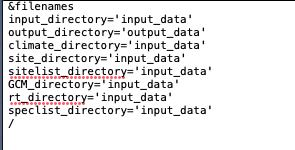
\includegraphics[width=0.6\linewidth]{manual_figures/filelist.png}
  \caption{Example of a \textit{file\_list.txt} file. As with all Fortran namelist files, the filelist file \textbf{must} start with ``\&filenames" (the name of the namelist in the model) and end with ``/". The parameters for the input/output directories (left side) should \textbf{not} be in quotes, whereas the path/name of the folder (right side) should be in quotes.}
  \label{fig:filelist}
\end{figure}

The directories within the file list should contain the input/output files as follows (see below for description of each file):
\begin{itemize}
\item \textbf{input\_directory}
	\begin{itemize}
	\item \textit{UVAFME2018\_rangelist.csv}
	\item \textit{UVAFME2018\_litterpars.csv}
	\end{itemize}
\item \textbf{output\_directory}
	\begin{itemize}
	\item All output files
	\end{itemize}
\item \textbf{climate\_directory}
	\begin{itemize}
	\item \textit{UVAFME2018\_climate.csv}
	\item \textit{UVAFME2018\_climate\_stddev.csv}
	\item \textit{UVAFME2018\_climate\_ex.csv}
	\item \textit{UVAFME2018\_climate\_ex\_stddev.csv}
	\item \textit{UVAFME2018\_lightning.csv}
	\end{itemize}
\item \textbf{site\_directory}
	\begin{itemize}
	\item \textit{UVAFME2018\_site.csv}
	\end{itemize}
\item \textbf{sitelist\_directory}
	\begin{itemize}
	\item \textit{UVAFME2018\_sitelist.csv}
	\end{itemize}
\item \textbf{GCM\_directory} (optional)
	\begin{itemize}
	\item \textit{UVAFME2018\_climate\_GCM.csv}
	\end{itemize}
\item \textbf{rt\_directory} 
	\begin{itemize}
	\item \textit{UVAFME2018\_runtime.txt}
	\end{itemize}
\item \textbf{speclist\_directory}
	\begin{itemize}
	\item \textit{UVAFME2018\_specieslist.csv}
	\end{itemize}
\end{itemize}

As in Fig. \ref{fig:filelist}, all input files may be in the same input directory, and thus all input directory parameters would be set to the same path/folder. However, these input files need not be in the same directory. The ability to break the input files up into separate directories allows for easier batch runs of multiple sites (see Section \ref{running}).

\subsubsection{Input files needed}
For a basic run, these ten files must be present in the appropriate input directory:

\begin{enumerate}
\item \textit{UVAFME2018\_runtime.txt}
\item \textit{UVAFME2018\_sitelist.csv}
\item \textit{UVAFME2018\_site.csv}
\item \textit{UVAFME2018\_rangelist.csv}
\item \textit{UVAFME2018\_specieslist.csv}
\item \textit{UVAFME2018\_climate.csv}
\item \textit{UVAFME2018\_climate\_stddev.csv}
\item \textit{UVAFME2018\_climate\_ex.csv}
\item \textit{UVAFME2018\_climate\_ex\_stddev.csv}
\item \textit{UVAFME2018\_lightning.csv}
\item \textit{UVAFME2018\_litterpars.csv}
\end{enumerate}

An optional \textit{UVAFME2018\_climate\_GCM.csv} file can be used for a non-linear climate change application (i.e. from a GCM file) (Section \ref{optional}). These files \textbf{must} have this exact naming convention or UVAFME will not recognize them and an I/O runtime error will occur.

\subsection{Description of Input Files}

\subsubsection{Runtime File}
The \textit{UVAFME2018\_runtime.txt} file sets up runtime parameters which are the same across all sites run. Such parameters include how many plots to simulate per site and their size, the number of years to run the simulations, as well as parameters for implementing climate change. The runtime file is a Fortran namelist file (Fig. \ref{fig:runtime}; see above description of filelist file). Thus, the parameter names in the input runtime file \textbf{must} match the parameter names set up inside the model or an I/O error will occur, and the default values for all subsequent parameters will be used. 

\begin{figure}
  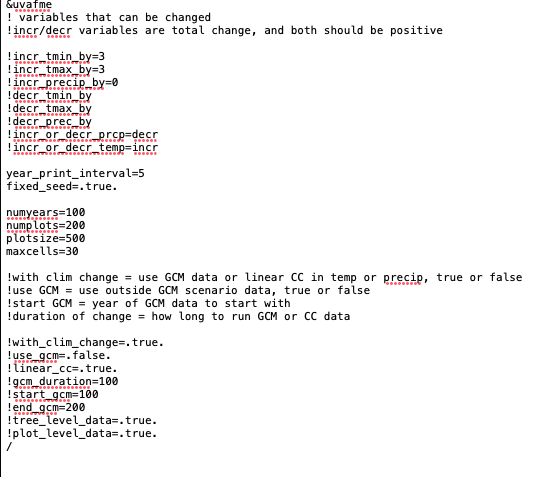
\includegraphics[width=0.6\linewidth]{manual_figures/UVAFME_Runtime.png}
  \caption{Example of a \textit{UVAFME2018\_runtime.txt} file. Lines that are commented out with a ``!" will not be read and those variables will take on the default parameters. As with all Fortran namelist files, the runtime file \textbf{must} start with ``\&uvafme" and end with ``/".}
  \label{fig:runtime}
\end{figure}

Runtime parameters that can be changed via the runtime file can be seen in Table \ref{tab:runtimetab}. The climate change-related parameters have checks intended to prevent unintended errors:
\begin{enumerate}
\item If using a climate change application (i.e. \textbf{with\_clim\_change} = TRUE) an error is thrown if the duration (i.e. \textbf{gcm\_duration}) is 0.0. 
\item If a linear climate change application is being used, an error is thrown if all of the \textbf{incr\_ } or \textbf{decr\_tmin/tmax/precip\_by} values are 0.0. 
\item Errors are thrown if \textbf{incr\_tmin\_by} or \textbf{incr\_tmax\_by} are negative when \textbf{incr\_or\_decr\_temp} is 'incr'.
\item Errors are thrown if \textbf{decr\_tmin\_by} or \textbf{decr\_tmax\_by} are 0.0 when \textbf{incr\_or\_decr\_temp} is 'decr'.
\item Errors are thrown if \textbf{incr\_precip\_by} is negative when \textbf{incr\_or\_decr\_precip} is 'incr'.
\item Errors are thrown if \textbf{decr\_precip\_by} is 0.0 when \textbf{incr\_or\_decr\_precip} is 'decr'.
\item The decrease-by values are intended to be input as positive values so if any \textbf{decr\_tmin/tmax/precip\_by} values are negative when a decrease is intended, then the value is changed to positive.
\end{enumerate}

Otherwise, for linear climate change applications, the annual temperature and precipitation change is calculated as:

\begin{equation}
 t' = \begin{cases}
 \frac{incr\_t\_by}{gcm\_duration + 1}, & \text{$incr\_or\_decr\_temp$ = `incr'} \\
\frac{-decr\_t\_by}{gcm\_duration + 1}, & \text{$incr\_or\_decr\_temp$ = `decr'} \\
\end{cases}
\end{equation}

and 

\begin{equation}
 p' = \begin{cases}
 \frac{incr\_precip\_by}{gcm\_duration + 1}, & \text{$incr\_or\_decr\_prcp$ = `incr'} \\
\frac{-decr\_precip\_by}{gcm\_duration + 1}, & \text{$incr\_or\_decr\_prcp$ = `decr'} \\
\end{cases}
\end{equation}

where $t'$ is the annual minimum or maximum temperature change (ºC), $p'$ is the annual precipitation change (proportional), and $incr\_t\_by$ and $decr\_t\_by$ are the overall linear \textbf{incr\_tmin/tmax\_by} or \textbf{decr\_tmin/tmax\_by} values. 

\begin{table}
\begin{center}
\caption{Parameters set up in runtime file.}
\label{tab:runtimetab}
\resizebox{\linewidth}{!}{%
\begin{tabular}{|c|c|c|} 
\hline
\textbf{Parameter Name} & \textbf{Description} & \textbf{Default Value}  \\
\hline 
\textbf{numplots} & number of plots to run per site &  200 \\
\hline 
\textbf{plotsize} & size of plot &  500 m$^2$ \\
\hline 
\textbf{year\_print\_interval} & interval at which to print output data & 10 years \\
\hline 
\textbf{maxcells} & maximum possible rows/columns for plot grid, maxcells*maxcells = maximum plants on plot &  100 \\
\hline
\textbf{maxtrees} & maximum trees on plot &  1000 \\
\hline
\textbf{maxshrubs} & maximum shrubs on plot &  9000 \\
\Xhline{5\arrayrulewidth}
\textbf{fixed\_seed} & \begin{tabular} {c} whether random seed is default (.true.) \\ or generated (.false.) \end{tabular} &  .false.\\
\hline
\textbf{debug} & debug flag related to random number generators &  .false.\\
\Xhline{5\arrayrulewidth}
\textbf{incr\_tmin\_by} & \begin{tabular} {c} amount to increase $\bar{t}_{min}$ \\ under linear climate change application \end{tabular} & 0.0 ºC \\
\hline 
\textbf{incr\_tmax\_by} & \begin{tabular} {c} amount to increase $\bar{t}_{max}$ \\ under linear climate change application \end{tabular} & 0.0 ºC\\
\hline 
\textbf{incr\_precip\_by} & \begin{tabular} {c} proportion to increase $\bar{p}$ \\ under linear climate change application \end{tabular} & 0.0 \\
\hline 
\textbf{decr\_tmin\_by} & \begin{tabular} {c} amount to decrease $\bar{t}_{min}$ \\ under linear climate change application \end{tabular} & 0.0 ºC \\
\hline 
\textbf{decr\_tmax\_by} &  \begin{tabular} {c} amount to decrease $\bar{t}_{max}$ \\ under linear climate change application \end{tabular} & 0.0 ºC \\
\hline 
\textbf{decr\_precip\_by} &  \begin{tabular} {c} proportion to decrease $\bar{p}$ \\ under linear climate change application \end{tabular} & 0.0 \\
\hline 
\textbf{incr\_or\_decr\_prcp} &  \begin{tabular} {c} whether or increase or decrease $\bar{p}$ \\ under linear climate change application \end{tabular} & `decr' \\
\hline 
\textbf{incr\_or\_decr\_temp} &  \begin{tabular} {c} whether or increase or decrease $\bar{t}$ \\ under linear climate change application \end{tabular} & `incr' \\
\hline 
\textbf{with\_clim\_change} & \begin{tabular} {c} whether or not to run \\ with climate change application \end{tabular} &  .false. \\
\hline 
\textbf{use\_gcm} & \begin{tabular} {c} whether or not to use an \\ input GCM file for climate \\ change application \end{tabular} &  .false. \\
\hline 
\textbf{linear\_cc} & \begin{tabular} {c}  whether or not to use a \\ linear climate change application \end{tabular} &  .false. \\
\hline 
\textbf{gcm\_duration} & the length of the climate change application &  0 years\\
\hline 
\textbf{start\_gcm} & the start year of the input GCM file &  0\\
\hline 
\textbf{end\_gcm} & the end year of the input GCM file & 100\\
\Xhline{5\arrayrulewidth}
\textbf{fire\_on} & whether to simulate fire &  .false.\\
\hline 
\textbf{fire\_tesing} & whether to force a fire at a specific time &  .false.\\
\Xhline{5\arrayrulewidth}
\textbf{use\_rangelist} & whether to use input rangelist &  .true.\\
\hline 
\textbf{use\_climstd} & whether to use input climate standard deviation file &  .true.\\
\hline
\textbf{tree\_level\_data} & whether to print out tree-level output data &  .false.\\
\hline 
\textbf{plot\_level\_data} & whether to print out plot-level output data &  .false.\\
\hline 
\textbf{testing} & whether to print out fine-scale fire and soil output &  .false.\\
\hline 
\textbf{conds\_testing} & whether to print out fine-scale fuel condition output data &  .false.\\
\hline
\textbf{reg\_testing} & whether to print out fine-scale regeneration output data &  .false.\\
\hline
\end{tabular}}
\end{center}
\end{table}

\subsubsection{Sitelist File}
The \textit{UVAFME2018\_sitelist.csv} file sets up the sites to be run in a simulation, as well as site-specific parameters such as the elevation of a site. While each of these parameters is generally also present in the site file (\textit{UVAFME2018\_site.csv}) or is a default parameter in the model, the setup here allows for sites to be parameterized with ``base" conditions in the Site file, and run with different parameters using the Sitelist file. This setup also allows the same site to be run multiple times with different parameters values (e.g. the s ame site run a multiple elevations). The Sitelist file must have the site IDs of each site to be run present in the \textbf{siteID} column, but all other columns may be left blank. Any other parameter left blank in the Sitelist file will take the values present in the Site file or default values in the model.

\begin{table}
\caption{Sitelist file parameters.}
\label{tab:sitelisttab}
\resizebox{\linewidth}{!}{%
\begin{tabular}{c|c|c|c} 
\textbf{Column Number} & \textbf{Column Name} & \textbf{Description} & \textbf{Units}\\
\hline 
1 & \textbf{siteID} & site ID for site - must include for runs & integer\\
2 & \textbf{runID} & run ID for site & integer\\
3 & \textbf{altitude} & altitude for site & meters\\
4 & \textbf{fire\_year} & stand age to force a fire & years\\
5 & \textbf{fire\_day} & day of year force a fire & Julian day\\
6 & \textbf{fire\_wind} & wind speed to force on day of fire & m s$^{-1}$\\
7 & \textbf{fire\_ffmc} & FFMC to force on day of fire & - \\
8 & \textbf{fire\_dmc} & DMC to force on day of fire & - \\
\end{tabular}}
\end{table}

\subsubsection{Specieslist File}
The \textit{UVAFME2018\_specieslist.csv} file contains the species-level parameters for each species to be simulated. These parameters include average maximum age, DBH, and height, tolerance levels to shade, drought and nutrients, and seedling/seedbank parameters (Table \ref{tab:specieslisttab}). Unless otherwise noted, most parameters are derived from a scientific literature review (e.g. \citeA{burnsSilvicsNorthAmerica1990}).

\begin{table}
\caption{Specieslist file parameters.}
\label{tab:specieslisttab}
\resizebox{\linewidth}{!}{%
\begin{tabular}{|c|c|c|c|c|} 
\hline
\textbf{Column Number} & \textbf{Column Name} & \textbf{Description} & \textbf{Units} & \textbf{Data Source}\\
\hline 
1 & \textbf{Group} & genus group number & integer & \\
\hline 
2 & \textbf{Genus} & genus of tree & character & \\
\hline 
3 & \textbf{Individual} & individual species number & integer & \\
\hline 
4 & \textbf{Scientific\_Name} & latin name of species & character & \\
\hline 
5 & \textbf{English\_Name} & common name of species & character &  \\
\hline 
6 & \textbf{form} & form of species (1 - tree; 2 - tree-like shrub; 3 - shrub; 4 - prostrate shrub ) & integer &  \\
\hline 
7 & \textbf{$AGE_{max}$} & average maximum age & years & \\
\hline 
8 & \textbf{$DBH_{max}$} & average maximum DBH & cm & \\
\hline
9 & \textbf{$H_{max}$} & average maximum height  & m & \\
\hline 
10 & \textbf{$rootdepth$} & average rooting depth  & m & \\
\hline 
11 & \textbf{$s$} & initial height-diameter relationship & m cm$^{-1}$ & \begin{tabular}{c} Equation A4 from \\ \citeA{botkinEcologicalConsequencesComputer1972} \\ (Fig. \ref{fig:sderiv} below) \end{tabular} \\
\hline 
12 & \textbf{$g$} & growth parameter & &  \begin{tabular}{c} Equation A4 from \\ \citeA{botkinEcologicalConsequencesComputer1972} \\ (Eq. \ref{gderiv} below) \end{tabular}\\
\hline 
13 & \textbf{$beta$} & stem shape parameter &  & \begin{tabular}{c} default 1.32 for coniferous; \\ 1.52 for broadleaf \end{tabular} \\
\hline 
14 & \textbf{bulk} & bulk density of wood & tonnes m$^{-3}$ & Miles and Smith 2008 \\
\hline 
15 & \textbf{$D_L$} & \begin{tabular} {c} Scalar parameter for \\ $LA~{D_{cbb}}^2$ relationship \end{tabular} &  & \begin{tabular}{c} default 0.184 for coniferous; \\ 0.175 for broadleaf \end{tabular}$^\text{§}$\\
\hline 
16 & \textbf{$LMA$} & leaf mass per area & tonnes C ha$^{-1}$ & \begin{tabular}{c} default 0.2 for coniferous; \\ 0.095 for broadleaf \end{tabular}  \\
\hline 
17 & \textbf{$GDD_{min}$} & \begin{tabular} {c} minimum degree day \\ threshold (5ºC base) \end{tabular} & degree-days & \\
\hline 
18 & \textbf{$GDD_{opt}$} & \begin{tabular} {c} optimum degree day \\ threshold (5ºC base) \end{tabular}  & degree-days &  \\
\hline
19 & \textbf{$GDD_{max}$} & \begin{tabular} {c} maximum degree day \\ threshold (5ºC base) \end{tabular}  & degree-days & \\
\hline 
20 & \textbf{shade} & relative shade tolerance & 1-5; 5 = least tolerant &\\
\hline 
21 & \textbf{drought} & relative drought tolerance & 1-6; 6 = least tolerant & \\
\hline 
22 & \textbf{flood} & relative inundation tolerance & 1-6; 6 = least tolerant & \\
\hline 
23 & \textbf{permf} & relative permafrost tolerance & 1-2; 2 = least tolerant & \\
\hline 
24 & \textbf{nutrient} & relative low nutrient tolerance & 1-3; 3 = least tolerant & \\
\hline
25 & \textbf{bark\_thick} & bark thickness per cm DBH & cm bark cm DBH$^{-1}$ & \citeA{keaneFireBGCv2LandscapeFire2011} \\
\hline 
26 & \textbf{$F_i$} & scorch height parameter & default 0.11 for needleleaf; 0.094 for broadleaf species & \\
\hline
27 & \textbf{fire\_regen} & \begin{tabular} {c} relative ability of plant to \\ resprout, regrow, or produce \\ seed after fire \end{tabular} & \begin{tabular} {c} 1-6;  \\ 1 = high reproduction \\ after fire; \\ 6 = low reproduction \\ after fire \end{tabular} & \\
\hline 
28 & \textbf{stress\_tol} & \begin{tabular} {c} relative ability to withstand \\ low growth from stress \end{tabular} & 1-5; 5 = least tolerant &\\
\hline 
29 & \textbf{death\_tol} & relative ability to live to AGE$_{max}$ & 1-3; 3 = least likely & \\
\hline 
30 & \textbf{dbh\_min} & minimum diameter increment growth before "stressed" & cm & \\
\hline 
31 & \textbf{evergreen} & evergreen or deciduous  & \begin{tabular} {c} evergreen = 1; \\ deciduous = 0 \end{tabular} &  \\
\hline 
32 & \textbf{litter\_class} & integer for litter class &  &  \\
\hline 
33 & \textbf{invader} & seed numbers from outside the plot  & seeds m$^{-2}$  & wind dispersed seeds = 1 \\
\hline 
34 & \textbf{seed} & seed numbers from within plot & seeds m$^{-2}$ & \begin{tabular} {c} e.g. cones $\approx$ 1; \\ samaras $\approx$ 10; \\ wind dispersed $\approx$ 100 \end{tabular} \\
\hline 
35 & \textbf{sprout} & \begin{tabular} {c} average sprouts produced \\ per individual \end{tabular} &  & \\
\hline 
36 & \textbf{layering} & \begin{tabular} {c} ability of species to \\ reproduce by layering \end{tabular} & 0 or 1 & \\
\hline 
37 & \textbf{org\_tol} & \begin{tabular} {c} relative ability of species to \\ reproduce on deep organic layers \end{tabular} & 1-3; 3 = least tolerant & \\
\hline 
38 & \textbf{recr\_age} & \begin{tabular} {c} age at which species \\ can reproduce \end{tabular} & years & \\
\hline 
39 & \textbf{min\_recr\_dbh} & \begin{tabular} {c} diameter at which species \\ can reproduce \end{tabular} & cm & \\
\hline
40 & \textbf{seed\_surv} & proportion seedbank lost annually & 0 to 1 & \\
\hline 
41 & \textbf{seedling\_surv} & \begin{tabular} {c} proportion seedling bank \\ lost annually \end{tabular} & 0 to 1  & \\
\hline 
42 & \textbf{species\_id} & \begin{tabular} {c} unique eight character code \\ consisting of first four letters \\ of genus and first four \\ letters of species \end{tabular} & & \\
\hline 
\multicolumn{5}{|c|}{\begin{tabular} {c} §: $D_L$ is further modified based on the species-specific shade tolerance (\textbf{shade}, $tol_{shade}$); $D_L = adj\times tol_{shade}$, \\ where $adj$ ranges from 1.5 to 1.7 depending on shade tolerance. \end{tabular}} \\
\hline
\end{tabular}}
\end{table}

To derive the parameters $s$ and $g$, equation A4 from \citeA{botkinEcologicalConsequencesComputer1972}  is used. For trees, the parameter $g$ is calculated using input parameters of $H_{max}$, $DBH_{max}$, and $AGE_{max}$:

\begin{equation} \label{gderiv}
g = \frac{4H_{max}}{AGE_{max}}\Bigg[\ln\Big(2(2DBH_{max} - 1)\Big) + \frac{\alpha}{2\ln(e_1)} - f\ln\Big(\frac{a \times c}{b \times d}\Big)\Bigg]
\end{equation}

where:

\begin{equation}
\alpha  =  1 - 1.37/H_{max}
\end{equation}

\begin{equation}
e_1 = \frac{\frac{9}{4} + 0.5\alpha}{(4DBH^2_{max} + 2\alpha DBH_{max}-\alpha)}
\end{equation}

\begin{equation}
a = 3 + \alpha - \sqrt{\alpha^2 + 4\alpha}
\end{equation}

\begin{equation}
 b = 3 + \alpha + \sqrt{\alpha^2 + 4\alpha}
\end{equation}

\begin{equation}
 c = 4DBH_{max} + \alpha + \sqrt{\alpha^2 + 4\alpha}
\end{equation}

\begin{equation}
d = 4DBH_{max} + \alpha - \sqrt{\alpha^2 + 4\alpha}
\end{equation}

and 

\begin{equation}
 f = \frac{\alpha + 0.5\alpha^2}{\sqrt{\alpha^2 + 4\alpha}}
\end{equation}

For shrubs, $g$ is derived as:

\begin{equation} \label{eq:gderiv_s}
	g = \frac{4H_{max}}{AGE_{max}}\Bigg[\ln\Big(2(2D_{max} - 1)\Big) + \frac{1}{2\ln(e_1)} - f\ln\Big(\frac{a \times c}{b \times d}\Big)\Bigg]
\end{equation}

where $D$ is the basal diameter (cm), $a = 1.763932$, $b = 6.236068$,  $c = 4D_{max} +  3.236068$, $d = 4D_{max} -1.236068$,
$f = 0.6708204$, and $e_1 = \frac{2.75}{(4D^2_{max} + 2D_{max}-1)}$.

The parameter $g$ is further modified within the model depending on shade tolerance, such that $g = g \times l$, where $l$ ranges from 1.1 to 1.25 depending on shade tolerance. The parameter $s$ is derived by regressing the initial height-diameter relationship calculated using Mitscherlich's equation (\citeA{botkinEcologicalConsequencesComputer1972}; Eq. \ref{mister}) with different $s$ values and that using a polynomial equation (Eq. \ref{poly}) until the slope of a line with y-intercept 0 is closest to 1.0 and the R$^2$ is closest to 1.0 (Fig. \ref{fig:sderiv}). 

For trees: 

\begin{equation} \label{mister}
H_m = 1.3 + (H_{max} - 1.3)(1 - \text{e}^{\frac{-sDBH}{H_{max} - 1.3}})
\end{equation}

\begin{equation} \label{poly}
H_p = (137 + b_2DBH - b_3DBH^2)/100
\end{equation}

where $b_2 = 2\frac{H_{max_{cm}} - 137}{DBH_{max}}$ and   $b_3 = \frac{H_{max_{cm}} - 137}{DBH^2_{max}}$.

For shrubs: 

\begin{equation} 
	H_m = (H_{max})(1 - \text{e}^{\frac{-sD}{H_{max}}})
\end{equation}

\begin{equation}
	H_p = (b_2D - b_3D^2)/100
\end{equation}

where $b_2 = 2\frac{H_{max_{cm}} }{D_{max}}$ and   $b_3 = \frac{H_{max_{cm}} }{D^2_{max}}$.

\begin{figure}[H]
  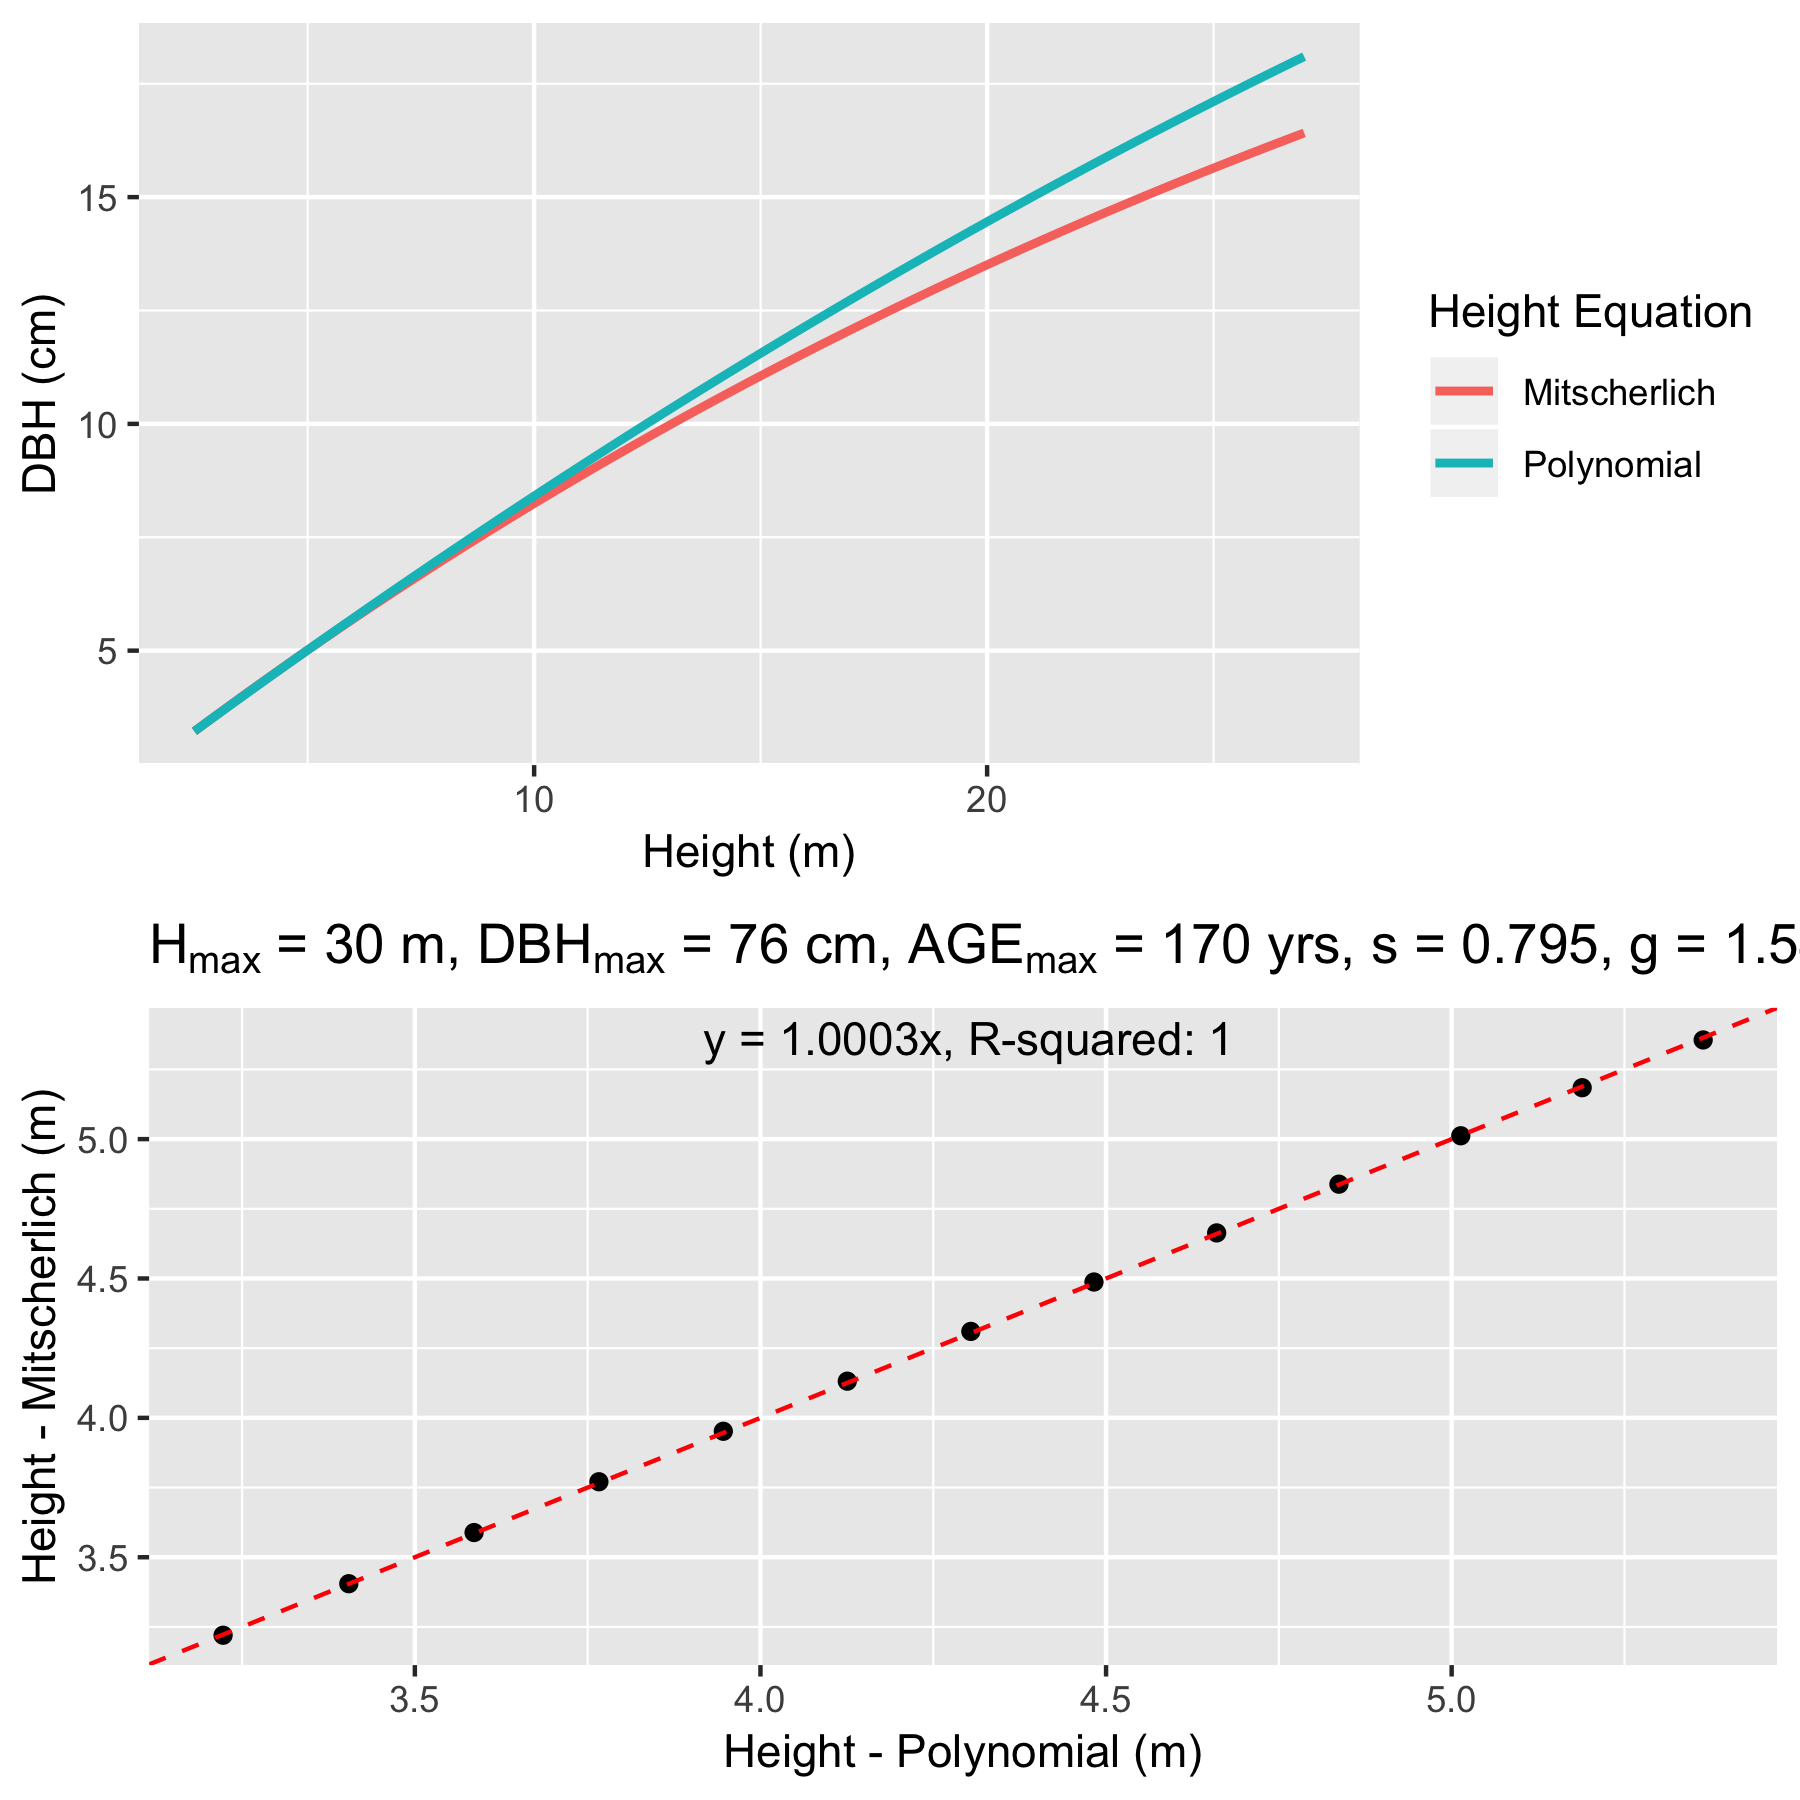
\includegraphics[width=0.8\linewidth]{manual_figures/Sderiv.png}
  \caption{Example derivation of parameter $s$ for a tree species with $H_{max}$ = 30 m, $DBH_{max}$ = 76 cm, and $AGE_{max}$ = 170 years.}
  \label{fig:sderiv}
\end{figure}

\subsubsection{Site File}
The \textit{UVAFME2018\_site.csv} file contains site-specific parameters for each site, including latitude, longitude, topography, soil characteristics, disturbance probabilities, and values for modifying temperature and precipitation if the elevation of the site is changed (i.e. climatic lapse rates) (Table \ref{tab:sitetab}). As with all other site-related files, the \textbf{siteID} column must match the site ids in all other files.

\begin{table}[H]
\caption{Site file parameters.}
\label{tab:sitetab}
\resizebox{\linewidth}{!}{%
\begin{tabular}{|c|c|c|c|c|} 
\hline
\textbf{Column Number} & \textbf{Column Name} & \textbf{Description} & \textbf{Units} & \textbf{Data Source}\\
\hline 
1 & \textbf{site} & unique site ID & integer  & user generated \\
\hline 
2 & \textbf{latitude} & latitude of site & decimal degrees & \\
\hline 
3 & \textbf{longitude} & longitude of site & decimal degrees & \\
\hline 
4 & \textbf{name} & site name & character & \\
\hline 
5 & \textbf{region} & region of site & character &  \\
\hline 
6 & \textbf{elevation} & elevation of site & meters & DEM \\
\hline 
7 & \textbf{slope} & slope of site & degrees & DEM \\
\hline
8 & \textbf{aspect} & aspect of site & degrees & DEM \\
\hline 
9 & \textbf{a\_sat} & saturation capacity of mineral layer & volumetric & site description; soil maps \\
\hline 
10 & \textbf{a\_fc} & field capacity of mineral layer  & volumetric & site description; soil maps\\
\hline 
11 & \textbf{a\_pwp} & permanent wilting point of mineral layer  & volumetric & site description; soil maps\\
\hline 
12 & \textbf{o\_sat} & saturation capacity of organic layer & volumetric & site description; soil maps \\
\hline 
13 & \textbf{o\_fc} & field capacity of organic layer  & volumetric & site description; soil maps\\
\hline 
14 & \textbf{o\_pwp} & permanent wilting point of organic layer  & volumetric & site description; soil maps\\
\hline 
15 & \textbf{a\_bd} & bulk density of mineral layer  & kg m$^{-3}$ & site description; soil maps\\
\hline 
16 & \textbf{o\_bd} & bulk density of organic layer  & kg m$^{-3}$ & site description; soil maps\\
\hline 
17 & \textbf{itxt} & soil texture &  \begin{tabular} {c} 0: very coarse \\ 1: coarse \\ 2: fine \end{tabular}  & site description; soil maps\\
\hline 
16 & \textbf{hum\_int} & initial humus amount  & t ha$^{-1}$ & site description; soil maps\\
\hline 
17 & \textbf{A\_depth} & depth of mineral (A) layer & m & site description; soil maps\\
\hline 
18 & \textbf{wind\_prob} & windthrow events in 1000 years & 1000/WRI & literature; site descriptions\\
\hline 
19 & \textbf{stand\_age} & simulation year to stop simulation & years & literature; site descriptions\\
\hline 
20 & \textbf{gcm\_year} & simulation year to start climate change & years & \\
\hline 
21 & \textbf{flow} & water input from overland flow & mm & \\
\hline 
\end{tabular}}
\end{table}

\subsubsection{Rangelist File}
The \textit{UVAFME2018\_rangelist.csv} file determines which species are eligible for colonization and growth at each site (Table \ref{tab:rangelisttab}). The column names are the species ids (8-character IDs set up in the \textit{UVAFME2018\_specieslist.csv} file), and the rows are each site. If a species is present at a site then the column/row will have a 1, and if the species is absent the column/row will have a 0. This is the only csv file where the column names are explicitly read by UVAFME and must match the species ids as set up in the Specieslist file. The order must also match the order of the Specieslist file. The presence/absence of each species is generally derived from species range maps (e.g. Little 1971) or site descriptions.

\begin{table}[H]
\caption{Rangelist file parameters.}
\label{tab:rangelisttab}
\resizebox{\linewidth}{!}{%
\begin{tabular}{|c|c|c|c|} 
\hline
\textbf{Column Number} & \textbf{Column Name} & \textbf{Description} & \textbf{Units} \\
\hline 
1 & \textbf{site} & unique site ID & integer \\
\hline 
2 & \textbf{latitude} & latitude of site & decimal degrees  \\
\hline 
3 & \textbf{longitude} & longitude of site & decimal degrees  \\
\hline 
4 ... n$_{\text{species}}$ & unique species ID & \begin{tabular} {c} presence or absence \\ of species at site \end{tabular} & \begin{tabular} {c} 0: absent; \\ 1: present \end{tabular} \\
\hline 
\end{tabular}}
\end{table}

\subsubsection{Climate Files}
The \textit{UVAFME2018\_climate.csv}, \textit{UVAFME2018\_climate\_stddev.csv}, \\
\textit{UVAFME2018\_climate\_ex.csv}, \textit{UVAFME2018\_climate\_ex\_stddev.csv}, and \textit{UVAFME2018\_lightning.csv} files contain the average and standard deviations of monthly minimum and maximum temperatures, precipitation, cloud cover, relative humidity, wind speed, and lightning strike density for each site (Tables \ref{tab:climatetab} - \ref{tab:lightningtab}). These data are generally derived from at least 30 years of historical climate data and are used to generate monthly and daily weather conditions within UVAFME.

\begin{table}[H]
\caption{\textit{UVAFME2018\_climate.csv} file parameters.}
\label{tab:climatetab}
\resizebox{\linewidth}{!}{%
\begin{tabular}{|c|c|c|c|} 
\hline
\textbf{Column Number} & \textbf{Column Name} & \textbf{Description} & \textbf{Units}\\
\hline 
1 & \textbf{site} & unique site ID & integer\\
\hline 
2 & \textbf{latitude} & latitude of site & decimal degrees \\
\hline 
3 & \textbf{longitude} & longitude of site & decimal degrees \\
\hline 
4 - 15 & \textbf{tmin\_[month]} & mean monthly minimum temperature & ºC \\
\hline 
16 - 27 & \textbf{tmax\_[month]} & mean monthly maximum temperature & ºC \\
\hline 
28 - 39 & \textbf{prcp\_[month]} & monthly precipitation & mm \\
\hline 
\end{tabular}}
\end{table}

\begin{table}[H]
\caption{\textit{UVAFME2018\_climate\_stddev.csv} file parameters.}
\label{tab:climatesdtab}
\resizebox{\linewidth}{!}{%
\begin{tabular}{|c|c|c|c|} 
\hline
\textbf{Column Number} & \textbf{Column Name} & \textbf{Description} & \textbf{Units}\\
\hline 
1 & \textbf{site} & unique site ID & integer\\
\hline 
2 & \textbf{latitude} & latitude of site & decimal degrees \\
\hline 
3 & \textbf{longitude} & longitude of site & decimal degrees \\
\hline 
4 - 15 & \textbf{tmin\_std\_[month]} & \begin{tabular} {c} standard deviation of \\ monthly minimum temperature \end{tabular} & ºC \\
\hline 
16 - 27 & \textbf{tmax\_std\_[month]} & \begin{tabular} {c} standard deviation of \\ monthly maximum temperature  \end{tabular} & ºC \\
\hline 
28 - 39 & \textbf{prcp\_std\_[month]} & \begin{tabular} {c} standard deviation of \\ monthly precipitation  \end{tabular} & mm \\
\hline 
\end{tabular}}
\end{table}

\begin{table}[H]
\caption{\textit{UVAFME2018\_ex\_climate.csv} file parameters.}
\label{tab:climateextab}
\resizebox{\linewidth}{!}{%
\begin{tabular}{|c|c|c|c|} 
\hline
\textbf{Column Number} & \textbf{Column Name} & \textbf{Description} & \textbf{Units}\\
\hline 
1 & \textbf{site} & unique site ID & integer\\
\hline 
2 & \textbf{latitude} & latitude of site & decimal degrees \\
\hline 
3 & \textbf{longitude} & longitude of site & decimal degrees \\
\hline 
4 - 15 & \textbf{cld\_[month]} & mean monthly cloudiness & \% sky covered \\
\hline 
16 - 27 & \textbf{rh\_[month]} & mean monthly relative humidity & \% \\
\hline 
28 - 39 & \textbf{wind\_[month]} & mean monthly wind speed & \ m s$^{-1}$ \\
\hline 
\end{tabular}}
\end{table}

\begin{table}[H]
\caption{\textit{UVAFME2018\_climate\_ex\_stddev.csv} file parameters.}
\label{tab:climateexsdtab}
\resizebox{\linewidth}{!}{%
\begin{tabular}{|c|c|c|c|} 
\hline
\textbf{Column Number} & \textbf{Column Name} & \textbf{Description} & \textbf{Units}\\
\hline 
1 & \textbf{site} & unique site ID & integer\\
\hline 
2 & \textbf{latitude} & latitude of site & decimal degrees \\
\hline 
3 & \textbf{longitude} & longitude of site & decimal degrees \\
\hline 
4 - 15 & \textbf{cld\_std\_[month]} & \begin{tabular} {c} standard deviation \\ of monthly cloudiness \end{tabular} & \% sky covered \\
\hline 
 16 - 27 & \textbf{rh\_std\_[month]} & \begin{tabular} {c} standard deviation \\ of monthly relative humidity \end{tabular} & \% \\
\hline 
\end{tabular}}
\end{table}

\begin{table}[H]
	\caption{\textit{UVAFME2018\_lightning.csv} file parameters.}
	\label{tab:lightningtab}
	\resizebox{\linewidth}{!}{%
		\begin{tabular}{|c|c|c|c|} 
			\hline
			\textbf{Column Number} & \textbf{Column Name} & \textbf{Description} & \textbf{Units}\\
			\hline 
			1 & \textbf{site} & unique site ID & integer\\
			\hline 
			2 & \textbf{latitude} & latitude of site & decimal degrees \\
			\hline 
			3 & \textbf{longitude} & longitude of site & decimal degrees \\
			\hline 
			4 - 15 & \textbf{strmn\_[month]} & mean monthly lightning strike density & strikes km$^{-2}$ day$^{-1}$ \\
			\hline 
			 16 - 27 & \textbf{strmn\_std\_[month]} & \begin{tabular} {c} standard deviation \\ of monthly lightning strike density \end{tabular} & strikes km$^{-2}$ day$^{-1}$ \\
			\hline 
	\end{tabular}}
\end{table}

\subsubsection{Litter Parameters File}
The \textit{UVAFME2018\_litterpars.csv} file contains the litter parameters used in the decomposition routine.

\begin{table}[H]
\caption{\textit{UVAFME2018\_litterpars.csv} file parameters. Parameter values are taken from \protect\citeA{bonanCarbonNitrogenCycling1990}, \protect\citeA{pastorDevelopmentLinkedForest1985}, and other available sources.}
\label{tab:littertab}
\resizebox{\linewidth}{!}{%
\begin{tabular}{|c|c|c|c|} 
\hline
\textbf{Column Number} & \textbf{Column Name} & \textbf{Description} & \textbf{Units}\\
\hline 
1 & \textbf{name} & cohort name & character\\
\hline 
2 & \textbf{InitialN} & initial N percent & 0 to 1 \\
\hline 
3 & \textbf{gImmob\_gwtloss} & \begin{tabular} {c} g N immobilized \\ per g weight loss \end{tabular} & g g$^{-1}$ \\
\hline 
4 & \textbf{critN} & \begin{tabular} {c} percent N at which \\ a decaying litter cohort is \\ transferred to well-decayed \\ wood or humus \end{tabular} & 0 to 1 \\
\hline 
5 & \textbf{litter\_type} & litter type ID & integer \\
\hline 
6 & \textbf{destination} & \begin{tabular} {c} if cohort is transferred to \\ well-decayed wood or humus \end{tabular} & \begin{tabular} {c} 1 = humus; \\ 2 = well-decayed wood \end{tabular} \\
\hline 
7 & \textbf{initialLignin} & initial percent lignin of cohort & 0 to 1\\
\hline 
8 & \textbf{ligParA} & lignin parameter $A$ & \\
\hline
9 & \textbf{ligParB} & lignin parameter $B$ & \\
\hline
10 & \textbf{Ash} & ash correction factor & 0 to 1 \\
\hline 
11 & \textbf{BD\_fresh} & bulk density of fresh litter & kg m$^{-3}$ \\
\hline 
12 & \textbf{SAV\_fresh} & surface area to volume ratio of fresh litter & cm$^{-1}$ \\
\hline 
\end{tabular}}
\end{table}

\subsection{Optional Input Files} \label{optional}

\subsubsection{Climate GCM File}

UVAFME has the option of applying climate change in the form of changing monthly minimum and maximum temperatures, precipitation, and lightning. The input files required for this application are the \\
 \textit{UVAFME2018\_climate\_GCM.csv} and  \textit{UVAFME2018\_lightning\_GCM.csv} files. Each contains the site ID, year, and monthly climate variables for each year of the climate change application (Tables \ref{tab:gcmtab} and \ref{tab:lightgcm}). Data for this file can be taken from output from earth system models or created by the user.

\begin{table}[H]
\caption{\textit{UVAFME2018\_climate\_GCM.csv} file parameters.}
\label{tab:gcmtab}
\resizebox{\linewidth}{!}{%
\begin{tabular}{|c|c|c|c|} 
\hline
\textbf{Column Number} & \textbf{Column Name} & \textbf{Description} & \textbf{Units}\\
\hline 
1 & \textbf{site} & unique site ID & integer\\
\hline 
2 & \textbf{latitude} & latitude of site & decimal degrees \\
\hline 
3 & \textbf{longitude} & longitude of site & decimal degrees \\
\hline 
4 & \textbf{year} & year of climate change application & integer \\
\hline 
5-16 & \textbf{tmin\_month} & mean monthly minimum temperature & ºC \\
\hline 
17-28 & \textbf{tmax\_month} & mean monthly maximum temperature & ºC \\
\hline 
29-40 & \textbf{prcp\_month} & mean monthly precipitation &  strikes km$^{-2}$ day$^{-1}$ \\
\hline 
\end{tabular}}
\end{table}

\begin{table}[H]
	\caption{\textit{UVAFME2018\_lightning\_GCM.csv} file parameters.}
	\label{tab:lightgcm}
	\resizebox{\linewidth}{!}{%
		\begin{tabular}{|c|c|c|c|} 
			\hline
			\textbf{Column Number} & \textbf{Column Name} & \textbf{Description} & \textbf{Units}\\
			\hline 
			1 & \textbf{site} & unique site ID & integer\\
			\hline 
			2 & \textbf{latitude} & latitude of site & decimal degrees \\
			\hline 
			3 & \textbf{longitude} & longitude of site & decimal degrees \\
			\hline 
			4 & \textbf{year} & year of climate change application & integer \\
			\hline 
			5-16 & \textbf{strmn\_month} & mean monthly lightning strike density & ºC \\
			\hline 
	\end{tabular}}
\end{table}


\section{Running the Model} \label{running}

To run UVAFME interactively from the command line simply enter: 

\newcommand\codeHighlight[1]{\textcolor[rgb]{1,0,0}{\textbf{#1}}}
\begin{Verbatim}[commandchars=\\\{\}]
./UVAFME_vx file_list.txt
\end{Verbatim}

This will run the model at each site specified in the Sitelist file, in order. Once the model has finished running, the output files will be in the \textbf{output\_data} directory. These output files will be rewritten every time the model is run, so be sure to save them elsewhere or with a different name (if desired) before re-running.

As mentioned above, the independence of the UVAFME sites allows for batches of sites to be distributed across several nodes of a computing cluster. This can be done iteratively, using different \textit{file\_list.txt} files which point the model to different input/output directories. It can also be accomplished using a job manager such as \href{https://slurm.schedmd.com/}{SLURM}.

\section{Model Outputs} \label{outputs}

\subsection{Standard Outputs}

\subsubsection{Species and Genus Output}

UVAFME outputs two standard files related to species- and genus-level forest characteristics, the \textit{Species\_Data.csv} file and the \textit{Genus\_Data.csv} file. For both files, at the specified year print interval (Section \ref{inputs}), the average (i.e. across plot) conditions for each species or genus are printed. If a species is specified as absent at a site in the input Rangelist file, the row is still printed but $-999$'s (i.e. the NA signifier) are printed in the data columns.

UVAFME also outputs  species- and genus-level files on the characteristics of trees that died each year, the \textit{Dead\_Species\_Data.csv} file and the \textit{Dead\_Genus\_Data.csv} file. For both files, at the specified year print interval (Section \ref{inputs}), the average (i.e. across plot) conditions for trees that died from each species or genus are printed. If a species is specified as absent at a site in the input Rangelist file, the row is still printed but $-999$'s are printed in the data columns.

\begin{table} [H]
\caption{\textit{Species\_Data.csv}  file output variables.}
\label{tab:outsptab}
\resizebox{\linewidth}{!}{%
\begin{tabular}{|c|c|c|c|} 
\hline
\textbf{Column Number} & \textbf{Column Name} & \textbf{Description} & \textbf{Units}\\
\hline 
1 & \textbf{siteID} & unique site ID & integer\\
\hline 
2 & \textbf{runID} & unique run ID & integer\\
\hline 
3 & \textbf{year} & simulation year & integer \\
\hline 
4 & \textbf{genus} & the genus of the species & character \\
\hline 
5 & \textbf{species} & the species ID & character \\
\hline 
6-16 & \textbf{[xx] to [xx]} & stem density in DBH bins & trees ha$^{-1}$ \\
\hline 
17-27 & \textbf{[xx] to [xx] biom} & biomass in DBH bins & tC ha$^{-1}$ \\
\hline 
28 & \textbf{degday\_resp} & growth response to temperature & 0 to 1\\
\hline 
29 & \textbf{drought\_resp} & growth response to drought & 0 to 1\\
\hline 
30 & \textbf{shade\_resp} & growth response to shade & 0 to 1\\
\hline 
31 & \textbf{perm\_resp} & growth response to permafrost & 0 to 1\\
\hline 
32 & \textbf{flood\_resp} & growth response to inundation & 0 to 1\\
\hline 
33 & \textbf{nutrient\_resp} & growth response to nutrients & 0 to 1\\
\hline 
34 & \textbf{max\_diam} & maximum DBH & cm\\
\hline 
35 & \textbf{mean\_diam} & average DBH & cm\\
\hline 
36 & \textbf{mean\_age} & average tree age & years\\
\hline 
37 & \textbf{max\_hgt} & maximum height & m\\
\hline 
38 & \textbf{leaf\_area\_ind} & leaf area index & m$^2$ m$^{-2}$\\
\hline 
39 & \textbf{basal\_area} & basal area & m$^2$ ha$^{-1}$ \\
\hline 
40 & \textbf{basal\_sd} & standard deviation of basal area & m$^2$ ha$^{-1}$ \\
\hline 
41 & \textbf{total\_biomC} & aboveground biomass & tC ha$^{-1}$ \\
\hline 
42 & \textbf{biomC\_sd} & standard deviation of aboveground biomass & tC ha$^{-1}$ \\
\hline 
43 & \textbf{biomC\_lg} & aboveground biomass of trees $\geq$ 9cm DBH & tC ha$^{-1}$ \\
\hline 
44 & \textbf{biomC\_std\_lg} & standard deviation of aboveground biomass of trees $\geq$9cm DBH & tC ha$^{-1}$ \\
\hline 
45 & \textbf{biomC\_sm} & aboveground biomass of trees $<$ 9cm DBH & tC ha$^{-1}$ \\
\hline 
46 & \textbf{biomC\_std\_sm} & standard deviation of aboveground biomass of trees $<$9cm DBH & tC ha$^{-1}$ \\
\hline 
47 & \textbf{basal\_lg} & basal area of trees $\geq$ 9cm DBH & m$^2$ ha$^{-1}$ \\
\hline 
48 & \textbf{basal\_std\_lg} & standard deviation of basal area of trees $\geq$ 9cm DBH & m$^2$  ha$^{-1}$ \\
\hline 
49 & \textbf{basal\_sm} & basal area of trees $<$ 9cm DBH & m$^2$  ha$^{-1}$ \\
\hline 
50 & \textbf{basal\_std\_sm} & standard deviation of basal area of trees $<$9cm DBH & m$^2$  ha$^{-1}$ \\
\hline 
51 & \textbf{dens\_lg} & stem density of trees $\geq$ 9cm DBH & trees ha$^{-1}$ \\
\hline 
52 & \textbf{dens\_std\_lg} & standard deviation of stem density of trees $\geq$ 9cm DBH & trees  ha$^{-1}$ \\
\hline 
53 & \textbf{dens\_sm} & stem density of trees $<$ 9cm DBH & trees ha$^{-1}$ \\
\hline 
54 & \textbf{dens\_std\_sm} & standard deviation of stem density of trees $<$ 9cm DBH & trees ha$^{-1}$ \\
\hline 
55 & \textbf{dbh\_lg} & average diameter of trees $\geq$ 9cm DBH & cm \\
\hline 
56 & \textbf{dbh\_std\_lg} & standard deviation of average diameter of trees $\geq$ 9cm DBH & cm \\
\hline 
57 & \textbf{dbh\_sm} & average diameter of trees $<$ 9cm DBH & cm \\
\hline 
58 & \textbf{dbh\_std\_sm} & standard deviation of average diameter of trees $<$ 9cm DBH & cm \\
\hline 
\end{tabular}}
\end{table}

\begin{table} [H]
\caption{\textit{Genus\_Data.csv}  file output variables.}
\label{tab:outgentab}
\resizebox{\linewidth}{!}{%
\begin{tabular}{|c|c|c|c|} 
\hline
\textbf{Column Number} & \textbf{Column Name} & \textbf{Description} & \textbf{Units}\\
\hline 
1 & \textbf{siteID} & unique site ID & integer\\
\hline 
2 & \textbf{runID} & unique run ID & integer\\
\hline 
3 & \textbf{year} & simulation year & integer \\
\hline 
4 & \textbf{genus} & the genus of the species & character \\
\hline 
5-15 & \textbf{[xx] to [xx]} & stem density in DBH bins & trees ha$^{-1}$ \\
\hline 
16-26 & \textbf{[xx] to [xx] biom} & biomass in DBH bins & tC ha$^{-1}$ \\
\hline 
27 & \textbf{degday\_resp} & growth response to temperature & 0 to 1\\
\hline 
28 & \textbf{drought\_resp} & growth response to drought & 0 to 1\\
\hline 
29 & \textbf{shade\_resp} & growth response to shade & 0 to 1\\
\hline 
30 & \textbf{perm\_resp} & growth response to permafrost & 0 to 1\\
\hline 
31 & \textbf{flood\_resp} & growth response to inundation & 0 to 1\\
\hline 
32 & \textbf{nutrient\_resp} & growth response to nutrients & 0 to 1\\
\hline 
33 & \textbf{max\_diam} & maximum DBH & cm\\
\hline 
34 & \textbf{mean\_diam} & average DBH & cm\\
\hline 
35 & \textbf{mean\_age} & average tree age & years\\
\hline 
36 & \textbf{max\_hgt} & maximum height & m\\
\hline 
37 & \textbf{leaf\_area\_ind} & leaf area index & m$^2$ m$^{-2}$\\
\hline 
38 & \textbf{basal\_area} & basal area & m$^2$ ha$^{-1}$ \\
\hline 
39 & \textbf{basal\_sd} & standard deviation of basal area & m$^2$ ha$^{-1}$ \\
\hline 
40 & \textbf{total\_biomC} & aboveground biomass & tC ha$^{-1}$ \\
\hline 
41 & \textbf{biomC\_sd} & standard deviation of aboveground biomass & tC ha$^{-1}$ \\
\hline 
42 & \textbf{biomC\_lg} & aboveground biomass of trees $\geq$ 9cm DBH & tC ha$^{-1}$ \\
\hline 
43 & \textbf{biomC\_std\_lg} & standard deviation of aboveground biomass of trees $\geq$9cm DBH & tC ha$^{-1}$ \\
\hline 
44 & \textbf{biomC\_sm} & aboveground biomass of trees $<$ 9cm DBH & tC ha$^{-1}$ \\
\hline 
45 & \textbf{biomC\_std\_sm} & standard deviation of aboveground biomass of trees $<$9cm DBH & tC ha$^{-1}$ \\
\hline 
46 & \textbf{basal\_lg} & basal area of trees $\geq$ 9cm DBH & m$^2$ ha$^{-1}$ \\
\hline 
47 & \textbf{basal\_std\_lg} & standard deviation of basal area of trees $\geq$ 9cm DBH & m$^2$  ha$^{-1}$ \\
\hline 
48 & \textbf{basal\_sm} & basal area of trees $<$ 9cm DBH & m$^2$  ha$^{-1}$ \\
\hline 
49 & \textbf{basal\_std\_sm} & standard deviation of basal area of trees $<$9cm DBH & m$^2$  ha$^{-1}$ \\
\hline 
50 & \textbf{dens\_lg} & stem density of trees $\geq$ 9cm DBH & trees ha$^{-1}$ \\
\hline 
51 & \textbf{dens\_std\_lg} & standard deviation of stem density of trees $\geq$ 9cm DBH & trees  ha$^{-1}$ \\
\hline 
52 & \textbf{dens\_sm} & stem density of trees $<$ 9cm DBH & trees ha$^{-1}$ \\
\hline 
53 & \textbf{dens\_std\_sm} & standard deviation of stem density of trees $<$ 9cm DBH & trees ha$^{-1}$ \\
\hline 
54 & \textbf{dbh\_lg} & average diameter of trees $\geq$ 9cm DBH & cm \\
\hline 
55 & \textbf{dbh\_std\_lg} & standard deviation of average diameter of trees $\geq$ 9cm DBH & cm \\
\hline 
56 & \textbf{dbh\_sm} & average diameter of trees $<$ 9cm DBH & cm \\
\hline 
57 & \textbf{dbh\_std\_sm} & standard deviation of average diameter of trees $<$ 9cm DBH & cm \\
\hline 
\hline 
\end{tabular}}
\end{table}

\begin{table} [H]
\caption{\textit{Dead\_Species\_Data.csv}  file output variables.}
\label{tab:outspdtab}
\resizebox{\linewidth}{!}{%
\begin{tabular}{|c|c|c|c|} 
\hline
\textbf{Column Number} & \textbf{Column Name} & \textbf{Description} & \textbf{Units}\\
\hline 
1 & \textbf{siteID} & unique site ID & integer\\
\hline 
2 & \textbf{runID} & unique run ID & integer\\
\hline 
3 & \textbf{year} & simulation year & integer \\
\hline 
4 & \textbf{genus} & the genus of the species & character \\
\hline 
5 & \textbf{species} & the species ID & character \\
\hline 
6 & \textbf{degday\_death} &  biomass of trees that died from temperature stress & tC ha$^{-1}$ \\
\hline 
7 & \textbf{drought\_death} &  biomass of trees that died from drought stress & tC ha$^{-1}$ \\
\hline 
8 & \textbf{shade\_death} &  biomass of trees that died from shade stress & tC ha$^{-1}$ \\
\hline 
9 & \textbf{perm\_death} &  biomass of trees that died from permafrost & tC ha$^{-1}$ \\
\hline 
10 & \textbf{flood\_death} &  biomass of trees that died from flooding inundation & tC ha$^{-1}$ \\
\hline 
11 & \textbf{nutrient\_death} &  biomass of trees that died from nutrient stress & tC ha$^{-1}$ \\
\hline
12 & \textbf{fire\_death} &  biomass of trees that died from wildfire & tC ha$^{-1}$ \\
\hline 
13 & \textbf{wind\_death} &  biomass of trees that died from windthrow & tC ha$^{-1}$ \\
\hline  
14 & \textbf{mean\_diam} & average DBH & cm\\
\hline 
15 & \textbf{total\_biomC} & average biomass & tC ha$^{-1}$ \\
\hline 
16 & \textbf{biomC\_sd} & standard deviation of biomass & tC ha$^{-1}$ \\
\hline 
\end{tabular}}
\end{table}

\begin{table} [H]
\caption{\textit{Dead\_Genus\_Data.csv}  file output variables.}
\label{tab:outgendtab}
\resizebox{\linewidth}{!}{%
\begin{tabular}{|c|c|c|c|} 
\hline
\textbf{Column Number} & \textbf{Column Name} & \textbf{Description} & \textbf{Units}\\
\hline 
1 & \textbf{siteID} & unique site ID & integer\\
\hline 
2 & \textbf{runID} & unique run ID & integer\\
\hline 
3 & \textbf{year} & simulation year & integer \\
\hline 
4 & \textbf{genus} & genus anme & character \\
\hline 
5 & \textbf{degday\_death} &  biomass of trees that died from temperature stress & tC ha$^{-1}$ \\
\hline 
6 & \textbf{drought\_death} &  biomass of trees that died from drought stress & tC ha$^{-1}$ \\
\hline 
7 & \textbf{shade\_death} &  biomass of trees that died from shade stress & tC ha$^{-1}$ \\
\hline 
8 & \textbf{perm\_death} &  biomass of trees that died from permafrost & tC ha$^{-1}$ \\
\hline 
9 & \textbf{flood\_death} &  biomass of trees that died from flooding inundation & tC ha$^{-1}$ \\
\hline 
10 & \textbf{nutrient\_death} &  biomass of trees that died from nutrient stress & tC ha$^{-1}$ \\
\hline 
11 & \textbf{fire\_death} &  biomass of trees that died from wildfire & tC ha$^{-1}$ \\
\hline 
12 & \textbf{wind\_death} &  biomass of trees that died from windthrow & tC ha$^{-1}$ \\
\hline 
13 & \textbf{mean\_diam} & average DBH & cm\\
\hline 
14 & \textbf{total\_biomC} & average biomass & tC ha$^{-1}$ \\
\hline 
15 & \textbf{biomC\_sd} & standard deviation of biomass & tC ha$^{-1}$ \\
\hline 
\end{tabular}}
\end{table}

\subsubsection{Across-Species/Genus Output}

UVAFME outputs a file related to across-species/genus forest characteristics, the \textit{Total\_Plot\_Values.csv} file. For this file, at the specified year print interval (Section \ref{inputs}), the average (i.e. across plot) conditions for all genera are printed. 

\begin{table} [H]
\caption{\textit{Total\_Plot\_Values.csv} file variables.}
\label{tab:outplottab}
\resizebox{\linewidth}{!}{%
\begin{tabular}{|c|c|c|c|} 
\hline
\textbf{Column Number} & \textbf{Column Name} & \textbf{Description} & \textbf{Units}\\
\hline 
1 & \textbf{siteID} & unique site ID & integer\\
\hline 
2 & \textbf{runID} & unique run ID & integer \\
\hline 
3 & \textbf{year} & simulation year & integer \\
\hline 
4 & \textbf{gdd\_death} & biomass loss due to low temperature stress  & tC ha$^{-1}$ \\
\hline 
5 & \textbf{drought\_death} & biomass loss due to drought stress  & tC ha$^{-1}$ \\
\hline 
6 & \textbf{shade\_death} & biomass loss due to shade stress  & tC ha$^{-1}$ \\
\hline 
7 & \textbf{perm\_death} & biomass loss due to permafrost stress  & tC ha$^{-1}$ \\
\hline 
8 & \textbf{flood\_death} & biomass loss due to flooding inundation  & tC ha$^{-1}$ \\
\hline 
9 & \textbf{nutrient\_death} & biomass loss due to low nutrient stress  & tC ha$^{-1}$ \\
\hline 
10 & \textbf{fire\_death} & biomass loss due to fire  & tC ha$^{-1}$ \\
\hline 
11 & \textbf{wind\_death} & biomass loss due to windthrow  & tC ha$^{-1}$ \\
\hline 
12 & \textbf{gddresp\_1} & growth response to temperature for trees 0-10 cm in DBH & 0 to 1 \\
\hline 
13 & \textbf{gddresp\_2} & growth response to temperature for trees 10-20 cm in DBH & 0 to 1 \\
\hline 
14 & \textbf{gddresp\_3} & growth response to temperature for trees 20-40 cm in DBH & 0 to 1 \\
\hline 
15 & \textbf{gddresp\_4} & growth response to temperature for trees 40+ cm in DBH & 0 to 1 \\
\hline
16 & \textbf{droughtresp\_1} & growth response to drought for trees 0-10 cm in DBHt & 0 to 1 \\
\hline 
17 & \textbf{droughtresp\_2} & growth response to drought for trees 0-20 cm in DBH & 0 to 1 \\
\hline 
18 & \textbf{droughtresp\_3} & growth response to drought for trees 20-40 cm in DBH & 0 to 1 \\
\hline 
19 & \textbf{droughtresp\_4} & growth response to drought for trees 40+ cm in DBH & 0 to 1 \\
\hline 
20 & \textbf{shaderesp\_1} & growth response to shade for trees 0-10 cm in DBH & 0 to 1 \\
\hline 
21 & \textbf{shaderesp\_2} & growth response to shade for trees 10-20 cm in DBH & 0 to 1 \\
\hline 
22 & \textbf{shaderesp\_3} & growth response to shade for trees 20-40 cm in DBH & 0 to 1 \\
\hline 
23 & \textbf{shaderesp\_4} & growth response to shade for trees 40+ cm in DBH & 0 to 1 \\
\hline 
24 & \textbf{permresp\_1} & growth response to permafrost for trees 0-10 cm in DBH & 0 to 1 \\
\hline 
25 & \textbf{permresp\_2} & growth response to permafrost for trees 0-20 cm in DBH & 0 to 1 \\
\hline 
26 & \textbf{permresp\_3} & growth response to permafrost for trees 20-40 cm in DBH & 0 to 1 \\
\hline 
27 & \textbf{permresp\_4} & growth response to permafrost for trees 40+ cm in DBH & 0 to 1 \\
\hline 
28 & \textbf{floodresp\_1} & growth response to inundation for trees 0-10 cm in DBH & 0 to 1 \\
\hline 
29 & \textbf{floodresp\_2} & growth response to inundation for trees 10-20 cm in DBH & 0 to 1 \\
\hline 
30 & \textbf{floodresp\_3} & growth response to inundation for trees 20-40 cm in DBH & 0 to 1 \\
\hline 
31 & \textbf{floodresp\_4} & growth response to inundation for trees 40+ cm in DBH & 0 to 1 \\
\hline 
32 & \textbf{nutrientresp\_1} & growth response to nutrients for trees 0-10 cm in DBH & 0 to 1 \\
\hline 
33 & \textbf{nutrientresp\_2} & growth response to nutrients for trees 0-20 cm in DBH & 0 to 1 \\
\hline 
34 & \textbf{nutrientresp\_3} & growth response to nutrients for trees 20-40 cm in DBH & 0 to 1 \\
\hline 
35 & \textbf{nutrientresp\_3} & growth response to nutrients for trees 40+ cm in DBH & 0 to 1 \\
\hline 
36 & \textbf{Loreys\_height} & average Loreys height  & m \\
\hline 
37 & \textbf{Loreys\_height\_sd} & standard deviation of Loreys height  & m \\
\hline 
38 & \textbf{max\_height} & average maximum height  & m \\
\hline 
39 & \textbf{max\_height\_sd} &  standard deviation of maximum height  & m \\
\hline 
40 & \textbf{total\_biomC} & average aboveground biomass & tC ha$^{-1}$ \\
\hline 
41 & \textbf{total\_biomC\_sd} &  standard deviation of biomass & tC ha$^{-1}$ \\
\hline 
42 & \textbf{basal\_area} & average basal area & m$^2$ ha$^{-1}$ \\
\hline 
43 & \textbf{basal\_area\_sd} & standard deviation of basal area & m$^2$ ha$^{-1}$ \\
\hline
44 & \textbf{total\_stems} & average stem density & trees ha$^{-1}$ \\
\hline 
45 & \textbf{total\_stems\_sd} & standard deviation of stem density & trees ha$^{-1}$ \\
\hline
46 & \textbf{small\_stems} & average stem density for trees $\leq$ 5 cm DBH & trees ha$^{-1}$ \\
\hline 
47 & \textbf{small\_stems\_sd} & standard deviation of stem density for trees $\leq$ 5 cm DBH & trees ha$^{-1}$ \\
\hline
48 & \textbf{med\_stems} & average stem density for trees $>$ 5 cm and $\leq$ 20 cm DBH & trees ha$^{-1}$ \\
\hline 
49 & \textbf{med\_stems\_sd} & standard deviation of stem density for trees $>$ 5 cm and $\leq$ 20 cm DBH & trees ha$^{-1}$ \\
\hline
50 & \textbf{lg\_stems} & average stem density for trees $>$ 20 cm DBH & trees ha$^{-1}$ \\
\hline 
51 & \textbf{lg\_stems\_sd} & standard deviation of stem density for trees $>$ 20 cm DBH & trees ha$^{-1}$ \\
\hline
52 & \textbf{stand\_age} &  average stand age & years \\
\hline 
53 & \textbf{stand\_age\_sd} &  standard deviation of stand age & years \\
\hline
54-65 & \textbf{LAI\_[1-12]} &  LAI in 5-m canopy sections (0-5...55-60) & m$^2$ m$^{-2}$ \\
\hline
\end{tabular}}
\end{table}

\subsubsection{Site and Climate Output}

UVAFME outputs a file related to climate and site characteristics, the \textit{Climate.csv} file. For this file, at the specified year print interval (Section \ref{inputs}), the several climate variables are printed out. Note output variables \textbf{thaw\_depth},
\textbf{organic\_depth}, \textbf{avail\_n}, \textbf{dryd\_upper} and \textbf{dryd\_lower} are averaged across all plots, all others are equal across all plots.

\begin{table} [H]
\caption{\textit{Climate.csv} file output variables.}
\label{tab:outclimtab}
\resizebox{\linewidth}{!}{%
\begin{tabular}{|c|c|c|c|} 
\hline
\textbf{Column Number} & \textbf{Column Name} & \textbf{Description} & \textbf{Units}\\
\hline 
1 & \textbf{siteID} & unique site ID & integer\\
\hline 
2 & \textbf{runID} & unique run ID & integer\\
\hline 
3 & \textbf{year} & simulation year & integer \\
\hline 
4 & \textbf{rain} & annual precipitation (snow and liquid) & cm \\
\hline 
5 & \textbf{pet} & annual potential evapotranspiration & cm \\
\hline 
6 & \textbf{solar\_rad} & annual surface solar radiation & cal cm$^2$ \\
\hline 
7 & \textbf{thaw\_depth} & active layer depth & cm \\
\hline 
8 & \textbf{organic\_depth} & organic layer depth & cm \\
\hline 
9 & \textbf{avail\_n} & plant-availble N & kgN ha$^{-1}$ \\
\hline 
10 & \textbf{aet} &  actual evapotranspiration & cm \\
\hline 
11 & \textbf{grow} & growing season length & days \\
\hline 
12 & \textbf{pc\_germ} & effect of temperature on black spruce regeneration & 0-1 \\
\hline 
13 & \textbf{degd} & growing degree-days & ºC-days \\
\hline 
14 & \textbf{drydays} & drought index & 0-1 \\
\hline 
15 & \textbf{saw0\_ByFC} & average mineral layer moisture scaled by field capacity &  \\
\hline 
16 & \textbf{saw0\_BySAT} & average mineral layer moisture scaled by saturation capacity &  \\
\hline 
17 & \textbf{aow0\_ByMin} & average organic layer moisture scaled by wilting point &  \\
\hline 
18 & \textbf{wilt\_days} & proportion of growing season below wilting point & 0-1 \\
\hline 
19 & \textbf{flood\_d} & proportion of growing season with flooded conditions & 0-1 \\
\hline 
\end{tabular}}
\end{table}

\subsubsection{Soil Output}

UVAFME outputs a file related to soil characteristics, the \textit{SoilDecomp.csv} file. For this file, at the specified year print interval (Section \ref{inputs}), the several soil-related variables are printed out, averaged across all plots. 

\begin{table} [H]
\caption{\textit{SoilDecomp.csv} file output variables.}
\label{tab:outsoiltab}
\resizebox{\linewidth}{!}{%
\begin{tabular}{|c|c|c|c|} 
\hline
\textbf{Column Number} & \textbf{Column Name} & \textbf{Description} & \textbf{Units}\\
\hline 
1 & \textbf{siteID} & unique site ID & integer\\
\hline 
2 & \textbf{runID} & unique run ID & integer\\
\hline 
3 & \textbf{year} & simulation year & integer \\
\hline 
4 & \textbf{odepth} & average organic layer depth & cm \\
\hline 
5 & \textbf{odepth\_sd} & standard deviation of organic layer depth & cm \\
\hline 
6 & \textbf{mdepth} & live moss depth & cm \\
\hline 
7 & \textbf{moss\_biom} & live moss biomass & kg ha$^{-1}$ \\
\hline 
8 & \textbf{active} & active layer depth & cm \\
\hline 
9 & \textbf{OM} & humus organic matter weight & t ha$^{-1}$ \\
\hline 
10 & \textbf{OM\_N} & organic matter N & tN ha$^{-1}$ \\
\hline 
11 & \textbf{lit\_cornus} & \textit{Cornus} leaf litter weight & t ha$^{-1}$  \\
\hline 
12 & \textbf{lit\_acerfrax} & \textit{Acer} and \textit{Fraxinus}  leaf litter weight & t ha$^{-1}$  \\
\hline 
13 & \textbf{lit\_prunus} & \textit{Prunus} leaf litter weight & t ha$^{-1}$  \\
\hline 
14 & \textbf{lit\_betula} &\textit{Betula} leaf litter weight & t ha$^{-1}$  \\
\hline 
15 & \textbf{lit\_queralba} & \textit{Quercus alba} leaf litter weight & t ha$^{-1}$  \\
\hline 
16 & \textbf{lit\_tsugthuj} & \textit{Tsuga} and  \textit{Thuja} leaf litter weight& t ha$^{-1}$  \\
\hline 
17 & \textbf{lit\_populus} & \textit{Populus} leaf litter weight & t ha$^{-1}$  \\
\hline 
18 & \textbf{lit\_fagus} & \textit{Fagus} leaf litter weight & t ha$^{-1}$  \\
\hline 
19 & \textbf{lit\_querrubr} & \textit{Quercus rubra} leaf litter weight& t ha$^{-1}$  \\
\hline 
20 & \textbf{lit\_abies} &\textit{Abies} leaf litter weight & t ha$^{-1}$  \\
\hline 
21 & \textbf{lit\_picea} & \textit{Picea} leaf litter weight & t ha$^{-1}$  \\
\hline 
22 & \textbf{lit\_pinus} & \textit{Pinus} leaf litter weight & t ha$^{-1}$  \\
\hline 
23 & \textbf{lit\_roots} & root litter cohort weight & t ha$^{-1}$  \\
\hline 
24 & \textbf{lit\_smboles} & small bole ($<$ 10 cm DBH) litter cohort weight  & t ha$^{-1}$  \\
\hline 
25 & \textbf{lit\_lboles} & large bole ($>$ 10 cm DBH)  litter cohort weight & t ha$^{-1}$  \\
\hline 
26 & \textbf{lit\_twigs} & twig litter cohort weight  & t ha$^{-1}$  \\
\hline 
27 & \textbf{lit\_smbranch} & small branch litter cohort weight  & t ha$^{-1}$  \\
\hline 
28 & \textbf{lit\_lbranch} & large branch litter cohort weight  & t ha$^{-1}$  \\
\hline 
29 & \textbf{lit\_WDW} & well-decayed wood litter cohort weight  & t ha$^{-1}$ \\
\hline 
30 & \textbf{lit\_moss} & moss litter cohort weight  & t ha$^{-1}$ \\
\hline 
31 & \textbf{avail\_n} & plant-available N & kgN ha$^{-1}$ \\
\hline 
\end{tabular}}
\end{table}

\subsubsection{Other Output Files}

UVAFME also outputs two text files, \textit{log.txt} and \textit{site\_log.txt}, that print messages regarding site and species data that are read in and initialized (for \textit{log.txt}) and whether each site run was successfully completed (for \textit{site\_log.txt}).  

For the \textit{log.txt} file, UVAFME will write ``Site data initialized. Total read in: [X]", where X is the number of sites read in from the site input file. It will also write ``Species data initialized. Total read in: [X]", where X is the number of species read in from the species parameter input file. Following this, it will write ``Species data initialized for site [X], where X is the site ID of each site run, each time the species data is initialized for that site. 

This file may also contain other messages if no climate data is found for a specific site: (e.g. ``No climate data for site number [X]". If any issues come up during runtime, the \textit{log.txt} file is a good first place to check. UVAFME also prints some error messages directly to the screen, especially if these errors cause the program to exit.

For the \textit{site\_log.txt} file, UVAFME will print ``Finished site [X]" (where X is the site ID) for each site it finished simulating. This file can be used to check to make sure all sites completed in a larger run.

\subsection{Optional Outputs}

\subsubsection{Plot-level Output}

UVAFME can optionally (see Section \ref{inputs}) output files which print plot-level species- and genus-level forest characteristics, the \textit{Plot\_Species\_Data.csv} and \textit{Plot\_Genus\_Data.csv} files. For these files, at the specified year print interval (Section \ref{inputs}), the plot conditions for trees from each species or genus are printed. If a species is specified as absent at a site in the input Rangelist file, the row is still printed but $-999$'s are printed in the data columns. Note: this will result in a lot of output data and will slow down your runs considerably, thus the plot\_level\_data flag in the runtime file should be used sparingly and only if necessary.

\begin{table} [H]
\caption{\textit{Plot\_Species\_Data.csv}  file output variables.}
\label{tab:outsppltab}
\resizebox{\linewidth}{!}{%
\begin{tabular}{|c|c|c|c|} 
\hline
\textbf{Column Number} & \textbf{Column Name} & \textbf{Description} & \textbf{Units}\\
\hline 
1 & \textbf{siteID} & unique site ID & integer\\
\hline 
2 & \textbf{runID} & unique run ID & integer\\
\hline 
3 & \textbf{year} & simulation year & integer \\
\hline 
4 & \textbf{plot} & plot number & integer \\
\hline 
5 & \textbf{genus} & the genus of the species & character \\
\hline 
6 & \textbf{species} & the species ID & character \\
\hline 
7-17 & \textbf{[xx] to [xx]} & stem density in DBH bins & trees ha$^{-1}$ \\
\hline 
18-28 & \textbf{[xx] to [xx] biom} & biomass in DBH bins & tC ha$^{-1}$ \\
\hline 
29 & \textbf{max\_diam} & maximum DBH & cm\\
\hline 
30 & \textbf{mean\_diam} & average DBH & cm\\
\hline  
31 & \textbf{max\_hgt} & maximum height & m\\
\hline 
32 & \textbf{leaf\_area\_ind} & leaf area index & m$^2$ m$^{-2}$ \\
\hline 
33 & \textbf{basal\_area} & basal area & m$^2$ ha$^{-1}$ \\
\hline 
34 & \textbf{total\_biomC} & biomass & tC ha$^{-1}$ \\
\hline 
\end{tabular}}
\end{table}

\begin{table} [H]
\caption{\textit{Plot\_Genus\_Data.csv}  file output variables.}
\label{tab:outgenpltab}
\resizebox{\linewidth}{!}{%
\begin{tabular}{|c|c|c|c|} 
\hline
\textbf{Column Number} & \textbf{Column Name} & \textbf{Description} & \textbf{Units}\\
\hline 
1 & \textbf{siteID} & unique site ID & integer\\
\hline 
2 & \textbf{runID} & unique run ID & integer\\
\hline 
3 & \textbf{year} & simulation year & integer \\
\hline 
4 & \textbf{plot} & plot number & integer \\
\hline 
5 & \textbf{genus} & genus name & character \\
\hline 
6-16 & \textbf{[xx] to [xx]} & stem density in DBH bins & trees ha$^{-1}$ \\
\hline 
17-27 & \textbf{[xx] to [xx] biom} & biomass in DBH bins & tC ha$^{-1}$ \\
\hline 
28 & \textbf{max\_diam} & maximum DBH & cm\\
\hline 
29 & \textbf{mean\_diam} & average DBH & cm\\
\hline  
30 & \textbf{max\_hgt} & maximum height & m\\
\hline 
31 & \textbf{leaf\_area\_ind} & leaf area index & m$^2$ m$^{-2}$ \\
\hline 
32 & \textbf{basal\_area} & basal area & m$^2$ ha$^{-1}$ \\
\hline 
33 & \textbf{total\_biomC} & biomass & tC ha$^{-1}$ \\
\hline 
\hline 
\end{tabular}}
\end{table}

If outputting plot-level data, UVAFME will also output plot-level species- and genus-level files on the characteristics of trees that died each year, the \textit{Plot\_Dead\_Species.csv} file and the \textit{Plot\_Dead\_Genus.csv} files. For both files, at the specified year print interval (Section \ref{inputs}), the individual plot conditions for trees that died from each species or genus are printed. If a species is specified as absent at a site in the input Rangelist file, the row is still printed but $-999$'s are printed in the data columns.

\begin{table} [H]
\caption{\textit{Plot\_Dead\_Species.csv}  file output variables.}
\label{tab:outspecpldtab}
\resizebox{\linewidth}{!}{%
\begin{tabular}{|c|c|c|c|} 
\hline
\textbf{Column Number} & \textbf{Column Name} & \textbf{Description} & \textbf{Units}\\
\hline 
1 & \textbf{siteID} & unique site ID & integer\\
\hline 
2 & \textbf{runID} & unique run ID & integer\\
\hline 
3 & \textbf{year} & simulation year & integer \\
\hline 
4 & \textbf{plot} & plot number & integer \\
\hline 
5 & \textbf{genus} & genus of species & character \\
\hline 
6 & \textbf{species} & unique species ID & character \\
\hline 
7 & \textbf{degday\_death} & biomass mortality due to temperature stress & tC ha$^{-1}$ \\
\hline 
8 & \textbf{drought\_death} & biomass mortality due to drought stress & tC ha$^{-1}$ \\
\hline 
9 & \textbf{shade\_death} & biomass mortality due to shade stress & tC ha$^{-1}$ \\
\hline 
10 & \textbf{perm\_death} & biomass mortality due to permafrost & tC ha$^{-1}$ \\
\hline 
11 & \textbf{flood\_death} & biomass mortality due to flooding inundation & tC ha$^{-1}$ \\
\hline 
12 & \textbf{nutrient\_death} & biomass mortality due to nutrient stress & tC ha$^{-1}$ \\
\hline 
13 & \textbf{fire\_death} & biomass mortality due to fire & tC ha$^{-1}$ \\
\hline 
14 & \textbf{wind\_death} & biomass mortality due to windthrow & tC ha$^{-1}$ \\
\hline 
15 & \textbf{mean\_diam} & average DBH & cm\\
\hline  
16 & \textbf{total\_biomC} & biomass & tC ha$^{-1}$ \\
\hline 
\end{tabular}}
\end{table}

\begin{table} [H]
\caption{\textit{Plot\_Dead\_Genus.csv}  file output variables.}
\label{tab:outgenpldtab}
\resizebox{\linewidth}{!}{%
\begin{tabular}{|c|c|c|c|} 
\hline
\textbf{Column Number} & \textbf{Column Name} & \textbf{Description} & \textbf{Units}\\
\hline 
1 & \textbf{siteID} & unique site ID & integer\\
\hline 
2 & \textbf{runID} & unique run ID & integer\\
\hline 
3 & \textbf{year} & simulation year & integer \\
\hline 
4 & \textbf{plot} & plot number & integer \\
\hline 
5 & \textbf{genus} & genus name & character \\
\hline 
6 & \textbf{degday\_death} & biomass mortality due to temperature stress & tC ha$^{-1}$ \\
\hline 
7 & \textbf{drought\_death} & biomass mortality due to drought stress & tC ha$^{-1}$ \\
\hline 
8 & \textbf{shade\_death} & biomass mortality due to shade stress & tC ha$^{-1}$ \\
\hline 
9 & \textbf{perm\_death} & biomass mortality due to permafrost & tC ha$^{-1}$ \\
\hline 
10 & \textbf{perm\_death} & biomass mortality due to flooding inundation & tC ha$^{-1}$ \\
\hline 
11 & \textbf{nutrient\_death} & biomass mortality due to nutrient stress & tC ha$^{-1}$ \\
\hline 
12 & \textbf{fire\_death} & biomass mortality due to fire & tC ha$^{-1}$ \\
\hline 
13 & \textbf{wind\_death} & biomass mortality due to windthrow & tC ha$^{-1}$ \\
\hline 
14 & \textbf{mean\_diam} & average DBH & cm\\
\hline  
15 & \textbf{total\_biomC} & biomass & tC ha$^{-1}$ \\
\hline 
\end{tabular}}
\end{table}

\subsubsection{Tree-level Output}

UVAFME can also optionally (see Section \ref{inputs}) output files which print tree-level characteristics for each plot, the \textit{Plot\_Tree\_Data.csv} file. For this file, at the specified year print interval (Section \ref{inputs}), 
tree characteristics for each plot are printed. Note: this will result in an even larger amount of output data and will slow down your runs considerably, thus the tree\_level\_data flag in the runtime file should be used extremely sparingly and only if necessary.

\begin{table} [H]
\caption{\textit{Plot\_Tree\_Data.csv}  file output variables.}
\label{tab:outtreetab}
\resizebox{\linewidth}{!}{%
\begin{tabular}{|c|c|c|c|} 
\hline
\textbf{Column Number} & \textbf{Column Name} & \textbf{Description} & \textbf{Units}\\
\hline 
1 & \textbf{siteID} & unique site ID & integer\\
\hline 
2 & \textbf{runID} & unique run ID & integer\\
\hline 
3 & \textbf{year} & simulation year & integer \\
\hline 
4 & \textbf{plot} & plot number & integer \\
\hline 
6 & \textbf{genus} & the genus of the tree & character \\
\hline 
7 & \textbf{species} & the species ID & character \\
\hline 
8 & \textbf{treeID} & the tree ID & character \\
\hline 
9 & \textbf{row} & the row location of the tree & integer \\
\hline 
10 & \textbf{col} & the column location of the tree & integer \\
\hline 
11 & \textbf{age} & age of tree & years \\
\hline 
12 & \textbf{diam} & diameter at breast height & cm\\
\hline 
13 & \textbf{dcbb} & diameter at clear branch bole height & cm\\
\hline 
14 & \textbf{height} & height & m\\
\hline  
15 & \textbf{cbb\_height} & clear branch bole height & m\\
\hline  
16 & \textbf{leaf\_biomass} & leaf biomass & tC \\
\hline 
17 & \textbf{leaf\_area} & leaf area & m$^2$ \\
\hline 
18 & \textbf{woody\_biomC} & aboveground woody biomass & tC \\
\hline 
19 & \textbf{degd\_resp} & growth response to temperature & 0-1 \\
\hline 
20 & \textbf{drought\_resp} & growth response to soil moisture & 0-1 \\
\hline 
21 & \textbf{shade\_resp} & growth response to shading & 0-1 \\
\hline 
22 & \textbf{perm\_resp} & growth response to permafrost & 0-1 \\
\hline 
23 & \textbf{flood\_resp} & growth response to flooding inundation & 0-1 \\
\hline 
24 & \textbf{nutrient\_resp} & growth response to nutrients & 0-1 \\
\hline 
\end{tabular}}
\end{table}

\subsubsection{Fuel conditions output}

UVAFME can also optionally (see Section \ref{inputs}) output a file which prints daily, plot-level fuel condition information, the \textit{Fuel\_Conds.csv} file. Note: this will result in an incredibly large amount of output data and will slow down your runs considerably, thus the conds\_testing flag in the runtime file should be used extremely sparingly and only if necessary.

\begin{table} [H]
	\caption{\textit{Fuel\_Conds.csv}  file output variables.}
	\label{tab:fuelconds}
	\resizebox{\linewidth}{!}{%
		\begin{tabular}{|c|c|c|c|} 
			\hline
			\textbf{Column Number} & \textbf{Column Name} & \textbf{Description} & \textbf{Units}\\
			\hline 
			1 & \textbf{siteID} & unique site ID & integer\\
			\hline 
			2 & \textbf{plot} & plot number & integer \\
			\hline 
			3 & \textbf{year} & simulation year & integer \\
			\hline 
		   	4  & \textbf{day} & day of year & integer \\
		   \hline 
			5 & \textbf{fuel\_sum} & total fuel loading  & kg m$^{-2}$  \\
			\hline 
			6 & \textbf{fuel\_dec} & fuel loading of deciduous leaf litter &  kg m$^{-2}$   \\
			\hline 
			7 & \textbf{fuel\_con} & fuel loading of needleleaf leaf litter  & kg m$^{-2}$  \\
			\hline 
			8 & \textbf{fuel\_twig} & fuel loading of twig litter   & kg m$^{-2}$   \\
			\hline 
			9 & \textbf{fuel\_smbr} & fuel loading of small branch litter  & kg m$^{-2}$   \\
			\hline 
			10 & \textbf{fuel\_lgbr} & fuel loading of large branch litter  & kg m$^{-2}$   \\
			\hline 
			11 & \textbf{fuel\_bole} & fuel loading of bole litter & kg m$^{-2}$   \\
			\hline 
			12 & \textbf{fuel\_moss} & fuel loading of live moss & kg m$^{-2}$   \\
			\hline 
			13 & \textbf{fuel\_dmoss} & fuel loading of moss litter & kg m$^{-2}$   \\
			\hline 
			14 & \textbf{fuel\_root} & fuel loading of root litter & kg m$^{-2}$   \\
			\hline 
			15 & \textbf{fuel\_shrub} & fuel loading of live shrubs &  kg m$^{-2}$  \\
			\hline 
			16 & \textbf{BD\_dec} & bulk density of deciduous leaf litter &  kg m$^{-3}$   \\
			\hline 
			17 & \textbf{BD\_con} &  bulk density of needleleaf leaf litter  & kg m$^{-3}$  \\
			\hline 
			18 & \textbf{BD\_twig} & bulk density of twig litter   & kg m$^{-3}$   \\
			\hline 
			19 & \textbf{BD\_smbr} & bulk density of small branch litter  & kg m$^{-3}$   \\
			\hline 
			20 & \textbf{BD\_lgbr} & bulk density of large branch litter  & kg m$^{-3}$   \\
			\hline 
			21 & \textbf{BD\_bole} & bulk density of bole litter & kg m$^{-3}$   \\
			\hline 
			22 & \textbf{BD\_moss} & bulk density of live moss & kg m$^{-3}$   \\
			\hline 
			23 & \textbf{BD\_dmoss} & bulk density of moss litter & kg m$^{-3}$   \\
			\hline 
			24 & \textbf{BD\_root} & bulk density of root litter & kg m$^{-3}$  \\
			\hline 
			25 & \textbf{BD\_shrub} & bulk density of live shrubs & kg m$^{-3}$  \\
			\hline 
			26 & \textbf{SAV\_dec} & surface area to volume ratio of deciduous leaf litter &  cm$^{-1}$   \\
			\hline 
			27 & \textbf{SAV\_con} &  surface area to volume ratio of needleleaf leaf litter  & cm$^{-1}$  \\
			\hline 
			28 & \textbf{SAV\_twig} & surface area to volume ratio of twig litter   & cm$^{-1}$   \\
			\hline 
			29 & \textbf{SAV\_smbr} & surface area to volume ratio of small branch litter  &cm$^{-1}$   \\
			\hline 
			30 & \textbf{SAV\_lgbr} & surface area to volume ratio of large branch litter  & cm$^{-1}$   \\
			\hline 
			31 & \textbf{SAV\_bole} & surface area to volume ratio of bole litter & cm$^{-1}$  \\
			\hline 
			32 & \textbf{SAV\_moss} & surface area to volume ratio of live moss & cm$^{-1}$   \\
			\hline 
			33 & \textbf{SAV\_dmoss} & surface area to volume ratio of moss litter & cm$^{-1}$   \\
			\hline 
			34 & \textbf{SAV\_root} & surface area to volume ratio of root litter & cm$^{-1}$  \\
			\hline 
			35 & \textbf{SAV\_shrub} & surface area to volume ratio of live shrubs & cm$^{-1}$  \\
			\hline 
			36 & \textbf{moist\_dec} & moisture of deciduous leaf litter &  m$^3$ m$^{-3}$   \\
			\hline 
			37 & \textbf{moist\_con} &  moisture of needleleaf leaf litter  & m$^3$ m$^{-3}$   \\
			\hline 
			38 & \textbf{moist\_twig} & moisture of twig litter   & m$^3$ m$^{-3}$   \\
			\hline 
			39 & \textbf{moist\_smbr} & moisture of small branch litter  & m$^3$ m$^{-3}$    \\
			\hline 
			40 & \textbf{moist\_lgbr} & moisture of large branch litter  & m$^3$ m$^{-3}$   \\
			\hline 
			41 & \textbf{moist\_bole} & moisture of bole litter & m$^3$ m$^{-3}$   \\
			\hline 
			42 & \textbf{moist\_moss} & moisture of live moss & m$^3$ m$^{-3}$    \\
			\hline 
			43 & \textbf{moist\_dmoss} & moisture of moss litter & m$^3$ m$^{-3}$   \\
			\hline 
			44 & \textbf{moist\_root} & moisture of root litter & m$^3$ m$^{-3}$   \\
			\hline 
			45 & \textbf{moist\_shrub} & moisture of live shrubs & m$^3$ m$^{-3}$   \\
			\hline 
			46 & \textbf{mef\_dec} & effective moisture of deciduous leaf litter &  0-1   \\
			\hline 
			47 & \textbf{mef\_con} &  effective moisture of needleleaf leaf litter  & 0-1     \\
			\hline 
			48 & \textbf{mef\_twig} & effective moisture of twig litter   & 0-1    \\
			\hline 
			49 & \textbf{mef\_smbr} & effective moisture of small branch litter  & 0-1      \\
			\hline 
			50 & \textbf{mef\_lgbr} & effective moisture of large branch litter  & 0-1    \\
			\hline 
			51 & \textbf{mef\_bole} & effective moisture of bole litter & 0-1     \\
			\hline 
			52 & \textbf{mef\_moss} & effective moisture of live moss & 0-1     \\
			\hline 
			53 & \textbf{mef\_dmoss} & effective moisture of moss litter & 0-1     \\
			\hline 
			54 & \textbf{mef\_root} & effective moisture of root litter & 0-1   \\
			\hline 
			55 & \textbf{mef\_shrub} & effective moisture of live shrubs & 0-1   \\
			\hline 
			56 & \textbf{sumlit\_moist} & moisture of total fuel & m$^3$ m$^{-3}$   \\
			\hline 
			57 & \textbf{sumlit\_SAV} & surface area to volume ratio of total fuel & cm$^{-1}$   \\
			\hline 
			58 & \textbf{sumlit\_BD} & bulk density of total fuel & kg m$^{-3}$   \\
			\hline 
			59 & \textbf{MEF} & effective moisture of total fuel &  0-1  \\
			\hline 
	\end{tabular}}
\end{table}

\subsubsection{Fire conditions output}

UVAFME can also optionally (see Section \ref{inputs}) output a file which prints plot-level fire condition information, the \textit{Fire\_Conds.csv} file. Every time a fire is ignited, this information is printed out.

\begin{table} [H]
	\caption{\textit{Fire\_Conds.csv}  file output variables.}
	\label{tab:fireconds}
	\resizebox{\linewidth}{!}{%
		\begin{tabular}{|c|c|c|c|} 
			\hline
			\textbf{Column Number} & \textbf{Column Name} & \textbf{Description} & \textbf{Units}\\
			\hline 
			1 & \textbf{siteID} & unique site ID & integer\\
			\hline 
			2 & \textbf{plot} & plot number & integer \\
			\hline 
			3 & \textbf{year} & simulation year & integer \\
			\hline 
			4  & \textbf{day} & day of year & integer \\
			\hline 
			5  & \textbf{FDI} & fire danger index & 0-1 \\
			\hline 
			6 & \textbf{ffmc} & fine fuel moisture code & -  \\
			\hline 
			7 & \textbf{MEF} & effective moisture of fuel &  0-1   \\
			\hline 
			8 & \textbf{fuel\_moisture} & moisture of fuel  & m$^3$  m$^{-3}$  \\
			\hline 
			9 & \textbf{fuel\_BD} & bulk density of fuel  & kg m$^{-3}$   \\
			\hline 
			10 & \textbf{fuel\_SAV} & surface area to volume ratio of fuel  & cm$^{-1}$   \\
			\hline 
			11 & \textbf{fuel\_dec} & fuel loading of deciduous leaf litter  & kg m$^{-2}$   \\
			\hline 
			12 & \textbf{fuel\_con} & fuel loading of needleleaf litter  & kg m$^{-2}$   \\
			\hline 
			13 & \textbf{fuel\_twig} & fuel loading of twig litter  & kg m$^{-2}$   \\
			\hline 
			14 & \textbf{fuel\_smbr} & fuel loading of small branch litter  & kg m$^{-2}$   \\
			\hline 
			15 & \textbf{fuel\_lgbr} & fuel loading of large branch litter  & kg m$^{-2}$   \\
			\hline 
			16 & \textbf{fuel\_bole} & fuel loading of bole litter & kg m$^{-2}$   \\
			\hline 
			17 & \textbf{fuel\_moss} & fuel loading of live moss & kg m$^{-2}$   \\
			\hline 
			18 & \textbf{fuel\_dmoss} & fuel loading of moss litter & kg m$^{-2}$   \\
			\hline 
			19 & \textbf{fuel\_root} & fuel loading of root litter & kg m$^{-2}$   \\
			\hline 
			20 & \textbf{fuel\_shrub} & fuel loading of live shrubs &  kg m$^{-2}$  \\
	        \hline
	        21 & \textbf{Uf} & effective wind speed &  m min$^{-1}$  \\
	        \hline
	        22 & \textbf{I\_r} & reaction intensity &  kJ kg$^{-1}$ m$^{-2}$  \\
	        \hline
	        23 & \textbf{flux\_rat} & propagating flux ratio &  -  \\
	        \hline
	        24 & \textbf{phi\_wind} & wind coefficient &  -  \\
	        \hline
	        25 & \textbf{Qig} & heat of pre-ignition &  kJ kg$^{-1}$  \\
	        \hline
	        26 & \textbf{rosf} & rate of spread &  m min$^{-1}$  \\
	        \hline
	        27 & \textbf{a\_f} & fire area &  ha \\
	        \hline
	        28 & \textbf{burn\_dec} & deciduous leaf litter consumed  & kg m$^{-2}$   \\
	        \hline 
	        29 & \textbf{burn\_con} & needleleaf litter consumed  & kg m$^{-2}$   \\
	        \hline 
	        30 & \textbf{burn\_twig} & twig litter consumed  & kg m$^{-2}$   \\
	        \hline 
	        31 & \textbf{burn\_smbr} & small branch litter consumed  & kg m$^{-2}$   \\
	        \hline 
	        32 & \textbf{burn\_lgbr} & large branch litter consumed  & kg m$^{-2}$   \\
	        \hline 
	        33 & \textbf{burn\_bole} & bole litter consumed & kg m$^{-2}$   \\
	        \hline 
	        34 & \textbf{burn\_moss} & live moss consumed & kg m$^{-2}$   \\
	        \hline 
	        35 & \textbf{burn\_dmoss} & moss litter consumed & kg m$^{-2}$   \\
	        \hline 
	        36 & \textbf{burn\_root} & root litter consumed & kg m$^{-2}$   \\
	        \hline 
	        37 & \textbf{burn\_shrub} & live shrubs consumed &  kg m$^{-2}$  \\
	        \hline 
	        38 & \textbf{I\_surf} & surface fire intensity &  kW m$^{-1}$  \\
	         \hline 
	        39 & \textbf{tau\_l} & residence time of fire & min  \\
	        \hline
	\end{tabular}}
\end{table}

\subsubsection{Fuel consumption output}

UVAFME can also optionally (see Section \ref{inputs}) output a file which prints plot-level fuel consumption information, the \textit{Cons\_Data.csv} file. Every time a fire burns fuel, this information is printed out.

\begin{table} [H]
	\caption{\textit{Cons\_Data.csv}  file output variables.}
	\label{tab:fireconds}
	\resizebox{\linewidth}{!}{%
		\begin{tabular}{|c|c|c|c|} 
			\hline
			\textbf{Column Number} & \textbf{Column Name} & \textbf{Description} & \textbf{Units}\\
			\hline 
			1 & \textbf{siteID} & unique site ID & integer\\
			\hline 
			2 & \textbf{plot} & plot number & integer \\
			\hline 
			3 & \textbf{year} & simulation year & integer \\
			\hline 
			5  & \textbf{dmc} & duff moisture code & - \\
			\hline 
			6 & \textbf{duff\_moist} & duff moisture & m$^3$  m$^{-3}$  \\
			\hline 
			7 & \textbf{rfs} & relative duff moisture content &  0-1   \\
			\hline 
			8 & \textbf{N\_cons} & proportion of N consumed by fire & 0-1   \\
			\hline 
			9 & \textbf{consRoot} & proportion of roots consumed by fire & 0-1    \\
			\hline 
			10 & \textbf{emis} & duff emissivity &    \\
			\hline 
			11 & \textbf{t\_r} & residence time of fire  & min  \\
			\hline 
			12 & \textbf{duff\_cons} & duff consumption through smoldering  & kg m$^{-2}$   \\
			\hline 
			13 & \textbf{hum\_avail} & humus content pre-fire & kg m$^{-2}$   \\
			\hline 
			14 & \textbf{pre\_depth} & depth of organic layer pre-fire & m  \\
			\hline 
			15 & \textbf{O\_depth} & depth of organic layer   & m  \\
			\hline 
			16 & \textbf{hum\_combust} & proportion humus consumed by fire & 0-1   \\
			\hline 
			17 & \textbf{bg\_combust} & belowground combustion & kg m$^{-2}$   \\
			\hline 
			18 & \textbf{agw\_combust} & aboveground woody combustion & kg m$^{-2}$   \\
			\hline 
			19 & \textbf{not\_burn} & live fuel that didn't burn & tC   \\
			\hline 
			20 & \textbf{canopy\_bd} & canopy bulk density  & kg m$^{-3}$   \\
			\hline 
			21 & \textbf{canopy\_bh} & canopy base height & m  \\
			\hline 
			22 & \textbf{canopy\_biom} & canopy biomass & kg m$^{-2}$   \\
			\hline 
			23 & \textbf{R\_a} & critical active rate of spread & m min$^{-1}$   \\
			\hline 
			24 & \textbf{rosf\_active} & active rate of spread & m min$^{-1}$   \\
			\hline 
			25 & \textbf{CFB} & crown fraction burnt & 0-1   \\
			\hline 
			26 & \textbf{R\_final} & final rate of spread & m min$^{-1}$   \\
			\hline 
			27 & \textbf{I\_final} & final fire intensity  & kW m$^{-1}$   \\
			\hline 
			28 & \textbf{abcombust} & aboveground combustion & tC  \\
			\hline 
			29 & \textbf{bgr\_combust} & root combustion & tC   \\
			\hline 
	\end{tabular}}
\end{table}

\section{Modifying UVAFME Code}

UVAFME source code files (.f90/.F90 files) can be modified using any text editing software. \href{https://www.geany.org}{Geany},  \href{https://help.gnome.org/users/gedit/stable/}{Gedit}, and \href{https://www.barebones.com/products/textwrangler/}{TextWrangler} are all good options that have Fortan-specific syntax highlighting. Once you have finished making changes you must recompile and remake the executable file. Recompiling requires a Fortran compiler (e.g., \href{https://software.intel.com/en-us/fortran-compilers}{ifort} or \href{https://gcc.gnu.org/wiki/GFortran}{gfortran}) .

Use the command ``\texttt{make}” within the source directory to make the new executable. Sometimes (especially if you have only made small changes) \textbf{ifort} doesn’t work very well and may not see all of the changes you have made. If you are having strange issues, try clearing all compiled files with the command ``\texttt{make clean}” before recompiling the whole model anew.

\textbf{Tip}: the UVAFME \textit{Makefile} (in the source code folder) can be changed as well. It may be especially useful to rename the executable (first line``\texttt{PROG = UVAFME\_v1\_NABoreal}”) for different versions so that you can keep track of all the different UVAFME versions (i.e.``\texttt{PROG = UVAFME\_fire}”, etc.). Then when you run this new executable you would simply replace the command \texttt{UVAFME\_v1} with your new executable name (i.e. ``\texttt{./UVAFME\_fire}”).

\section{Tips and Tricks} \label{tips}

Below are some common errors that may occur when running UVAFME and modifying input files and source code.

\subsubsection{Column Names and Order}
Except for the Rangelist file, UVAFME \textbf{\textit{does not}} read the column headers for the input csv files. This means that if your order is not exactly correct (see above sections) UVAFME will read in variables incorrectly, but show no errors (though an error should occur if UVAFME reads in a variable type it is not expecting, i.e. a character when it is expecting a real). Make sure the column order in your input files exactly matches the above tables. This also means that you can change the column names for all but the Rangelist file as you see fit.

\subsubsection{NAs in Sitelist File}
Though most of the columns (i.e. all but the \textbf{siteID} column) may be left blank in the \textit{UVAFME2018\_sitelist.csv} file, make sure they are not written as NA/NaN's, etc. They must be blank or UVAFME will not be able to read the file and this error will be thrown:

\begin{figure}[ht]
  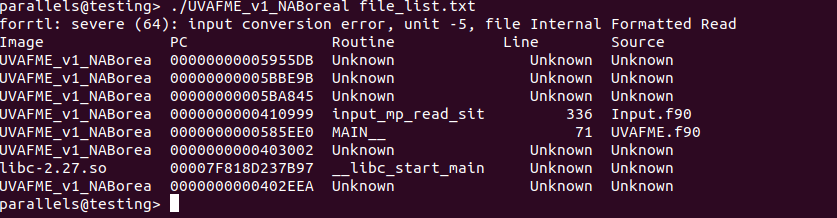
\includegraphics[width=\linewidth]{manual_figures/Terminal_NAs.png}
\end{figure}

\subsubsection{Rangelist File}
As stated in Section \ref{inputs}, the \textit{UVAFME2018\_rangelist.csv} file is the only csv file where the column \textbf{names} are specifically read in by UVAFME and used to compare to the species IDs set up in the Specieslist file. This means that these column names \textbf{cannot} be in quotes or an error will occur. If using a software such as \textbf{R} to create the Rangelist file, be sure to write the file without quotes in the column names. If quotes are present, the model will determine that no species are present at the sites and will skip all sites, diplaying the warning message:
\\

\begin{verbcode}
No species present in site  <siteID>
Skipping site <site name>
\end{verbcode}

\subsubsection{End of Line Issues}
If you have I/O errors and aren’t sure what is going on (especially if you have a Mac) you may have an end of line issue. The Mac version of MS Excel does not communicate well with Fortran. If you modify any .csv files on a Mac MS Excel, be sure to save them as ``Windows Comma Separated,” which should solve end of line issues.

\subsubsection{Adding Object Attributes}
Currently, sometimes errors arise when a new attribute is added to an object (i.e. a new attribute is added to the \textbf{Plot} object; see \textit{Plot.f90}). It seems that \textbf{ifort} doesn't always catch these additions and then memory-related issues arise. A simple solution when these errors occur is to ``\texttt{make clean}" the entire source code folder and recompile all files.

\subsubsection{Everything Else...}
Otherwise, if you cannot determine what is wrong, you can add the \\
``\texttt{-traceback}” flag to the \texttt{DBG} line in the UVAFME \textit{Makefile}. This will give you the exact line number and module where the error occurred, and is sometimes very helpful in finding errors. Be sure to take this flag out when you are finished debugging as it adds a lot of time to runs.

\bibliographystyle{apacite} 
 \bibliography{ReferencesNew}

\end{document}